% Learn Go with Pocket-Sized Projects — Chapter 11
\chapter{使用 gRPC 客户端渲染 HTML 模板}

\begin{infobox}{本章内容}
\begin{itemize}
  \item 创建 gRPC 客户端
  \item 使用 Go 模板填充 HTML 页面
  \item 调用现有后端服务
\end{itemize}
\end{infobox}

手里有一批数据想要展示时，首先得回答两个主要问题：展示什么，以及怎样展示。回答第一个问题，属于理解问题本身的一部分；而知道该怎样呈现结果、怎样把它讲清楚，往往又是让解决方案真正有意义的必要条件。身为计算机从业者，我们每天都在处理海量数据，其中大部分在邻居、学校里其他孩子的家长，或超市收银队伍里站在前面那个人眼中，都平淡得不能再平淡。第 5 章讲过，图标如何让 Wordle——以及我们自己的 Gordle——比一串单纯的数字更有趣。清楚地呈现原始数据如此重要，以至于 Go 开发者在语言的第一个版本中就加入了 \texttt{text/template} 包来支持这件事。这个包和它的姊妹包 \texttt{html/template}，目的都是依据数据内容生成更丰富的文本输出。多数时候，数据还需要精心排版：这里添一个制表符，那里插一处换行，再补上这个或那个标签。本章也会说明，为什么 Go 的其他工具通常不如模板适合这项工作。

Helm 等工具大量使用模板，把 YAML 部署配置文件中重复的部分抽取出来，使配置更加通用。本章将使用 Go 的模板包，在上一章编写的习惯追踪器之上搭建一套好看的用户界面。为此，我们要与一个 Web 服务器交互；它会显示一张 HTML 页面，其中包含与习惯有关的重要信息。说到底，\texttt{grpcurl} 的确好用，但按钮带来的体验显然更佳——哪怕只是为了测试！本项目需要满足以下要求：

\begin{itemize}
  \item 用户必须能通过 Web 浏览器访问 HTTP 服务器；
  \item Web 页面要以赏心悦目的方式展示当前习惯；
  \item 用户可以在页面中为本周的某项习惯打卡，也可以创建新习惯；
  \item HTTP 服务器要与我们的 gRPC 习惯服务通信；
  \item HTTP 服务器返回一份包含习惯信息的 HTML 文档。
\end{itemize}

\begin{infobox}{阅读提示}
本章依赖第 10 章的代码。如果你跳过了上一章，可以使用本书代码仓库中提供的实现。
\end{infobox}

\section{搭建基础 HTTP 服务器}

先看图 \ref{fig:ch11-architecture}，从整体上理解本章目标。目前，我们已经实现了 gRPC 习惯服务和存储逻辑；接下来还需要一台 HTTP 服务器，把内容转换成美观的 HTML 页面，再把页面提供给用户的 Web 浏览器。

\begin{figure}[tbp]
  \centering
  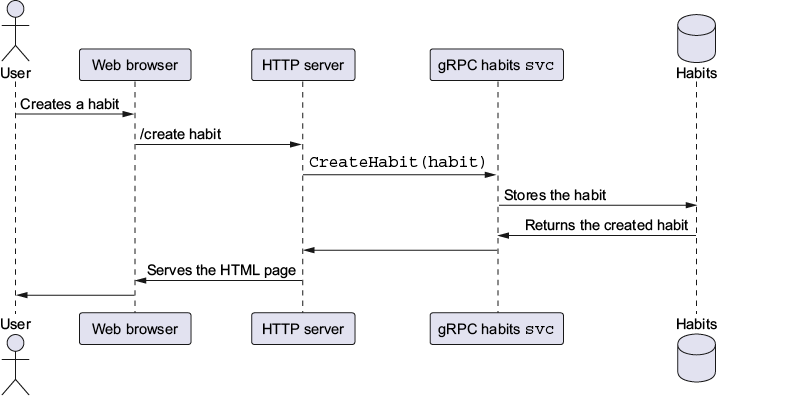
\includegraphics[width=0.96\textwidth]{figures/ch11/CH11_F01_Latour.png}
  \caption{系统总体架构的 UML 图}
  \label{fig:ch11-architecture}
\end{figure}

第一步，是运行一台能够向 Web 浏览器返回 HTML 的服务器。不过先别急着写 HTML：先让服务器返回点东西，确认它能工作。这相当于 HTTP 世界里的 \texttt{hello, world}，位于服务根路径 \url{http://localhost:8083/}。端口可以自行选择；开发期间，\texttt{8080} 及以上通常是不错的范围。这台服务器会成为一座桥梁：接收用户正在浏览的 Web 页面发来的 HTTP 请求，再向另一侧的 gRPC 服务器发送恰当的 Protobuf 消息。

第 8 章已经介绍过 HTTP 服务器的基础，这里快速回顾一遍。新建目录并初始化模块：运行 \texttt{go mod init learngo-pockets/templates}，或者使用其他模块名；随后在 \path{cmd/httpserver} 中创建 \texttt{main.go}。这样一台服务器只需寥寥几行。

\begin{gocode}[title={代码清单 11.1 最小 HTTP 服务器}]
func main() {
    http.HandleFunc("/",
        func(w http.ResponseWriter, r *http.Request) { #1
            io.WriteString(w, "ሰላም፣ሰዎች።") #2
        })

    err := http.ListenAndServe(":8083", nil) #3
    if err != nil {
        fmt.Fprintln(os.Stderr,
            "Error while serving: "+err.Error())
    }
}
\end{gocode}

\begin{codeannotations}
\item 为根路径 \texttt{/} 定义处理函数
\item 页面内容
\item 在端口 \texttt{8083} 启动 HTTP 服务器
\end{codeannotations}

运行程序，打开浏览器并访问 \url{http://localhost:8083}。浏览器显示页面时，会向本机端口 \texttt{8083} 发出请求；服务器在那里接收请求，并返回 \texttt{“ሰላም፣ሰዎች።”}——这是阿姆哈拉语的“你好，世界。”，而且其中的逗号和句号并不是英文里的 \texttt{,} 与 \texttt{.} 字符。浏览器随后接收并显示响应。可以执行下面的命令，再打开上述地址：

\begin{shellcode}[]
> go run cmd/httpserver/main.go
\end{shellcode}

看到消息了吗？接下来把代码整理得更便于后来维护。

\subsection{先输出纯文本}

当然，这种扁平的代码结构走不了多远。趁代码还没长大，先把它组织起来。沿用第 8 章的选择，创建 \texttt{internal/handlers} 包，把“某条路径被请求时该做什么”的逻辑放进去。在传统的纯 HTML 网站中，默认显示的页面通常称为 \emph{index}，这里继续使用这个名字。分别创建保存服务器结构和主页逻辑的文件：

\begin{treebox}
\PocketTreeLine{.}
\PocketTreeLine{├── cmd}
\PocketTreeLine{│   └── httpserver}
\PocketTreeLine{│       └── main.go}
\PocketTreeLine{├── go.mod}
\PocketTreeLine{├── go.sum}
\PocketTreeLine{└── internal}
\PocketTreeLine{    └── handlers}
\PocketTreeLine{        ├── index.go}
\PocketTreeLine{        └── server.go}
\end{treebox}

\subsubsection{main 函数}

先更新 \texttt{main}：创建服务器，再用它的路由器监听并处理请求，如代码清单 11.2 所示。服务器本身下一步再实现。你会发现，监听端口和提供服务的方式与前面那个直截了当的版本相同，变化只有路由器参数：我们希望所有路由都由接下来编写的服务器统一管理。

\begin{gocode}[title={代码清单 11.2 \texttt{main.go}：使用服务器的路由器}]
const port = 8083

func main() {
    srv := handlers.New() #1

    addr := fmt.Sprintf(":%d", port)
    // TODO: Log a message: we are listening

    err := http.ListenAndServe(addr, srv.Router()) #2
    if err != nil {
        panic(err)
    }
}
\end{gocode}

\begin{codeannotations}
\item 创建服务器——此时代码还不能编译
\item 监听端口 \texttt{8083}
\end{codeannotations}

编译器不开心，开发者也不会开心，所以现在实现这台服务器。

\subsubsection{服务器结构}

照例，我们希望服务器是一份保存依赖的结构体，这样就能配合相应 mock 进行测试。在把 gRPC 客户端加入依赖之前，这个结构首先需要一项功能：构建路由器，把不同端点连接起来。第 8 章已经解释过，为什么选择标准库而不是 \texttt{go-chi}、\texttt{fiber} 或 \texttt{gorilla} 作为路由库；这里继续保持同样选择。先写一个空的 \texttt{Server} 结构，并添加暂时不接收参数的 \texttt{New()} 函数，再实现路由器。

\begin{gocode}[title={代码清单 11.3 \texttt{server.go}：\texttt{Server} 结构}]
// Server serves all the HTML routes on this service.
type Server struct{} #1

func New() *Server { #2
    return &Server{}
}

// Router returns an HTTP handler that listens to all the proper paths.
func (s *Server) Router() http.Handler {
    r := http.NewServeMux() #3

    // Register each endpoint.
    r.HandleFunc(http.MethodGet+" "+"/", s.index) #4

    return r
}
\end{gocode}

\begin{codeannotations}
\item 定义空结构
\item 实现 \texttt{New}
\item 创建服务器路由器
\item 把 \texttt{s.index} 处理器注册到 \texttt{GET /}
\end{codeannotations}

每一张页面、每一个端点或路径，都将由 \texttt{Server} 结构上的方法处理。现在要实现 \texttt{index}，负责服务器根路径。

\subsubsection{主页}

客户端导航到主页时，究竟要运行什么逻辑？根据上一份代码清单，服务器知道应该调用 \texttt{index} 方法；这个方法需要返回状态码和页面内容。

查看文档可知，\texttt{HandleFunc} 按指定 HTTP 动词声明路由，并把请求交给第二个参数——一份 \texttt{http.HandlerFunc}。因此，\texttt{index} 必须使用文档规定的特定签名：

\begin{gocode}[]
// The HandlerFunc type is an adapter to allow the use of
// ordinary functions as HTTP handlers.
// [...]
type HandlerFunc func(ResponseWriter, *Request)
\end{gocode}

在独立文件中——例如 \texttt{index.go}——用这个签名写出 \texttt{index}：

\begin{gocode}[]
// index serves the root page of the app.
func (*Server) index(w http.ResponseWriter, r *http.Request) {}
\end{gocode}

这个函数眼下只需要完成一项操作：把一些 HTML 写入变量 \texttt{w}。该用 \texttt{fmt.Fprint}，还是 \texttt{io.WriteString}？向 writer 写字符串主要有两组选择：\texttt{io.WriteString(w, ...)}，或者 \texttt{fmt.Fprint(w, ...)} 系列。若内容是一条硬编码字符串，\texttt{WriteString} 再合适不过；但一旦要往字符串中加入信息、使它动态变化，通常就需要 \texttt{fmt} 包。弄清这一点后，再输出一次“Hello, World”，看看重构后是否仍然正常。

\begin{gocode}[title={代码清单 11.4 \texttt{index.go}：主页处理器}]
// index serves the root page of the app.
func (_ *Server) index(w http.ResponseWriter, _ *http.Request) {
    io.WriteString(w, "ሰላም፣ሰዎች።")
}
\end{gocode}

\begin{figure}[tbp]
  \centering
  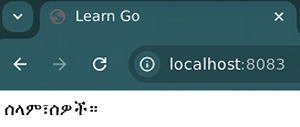
\includegraphics[width=0.58\textwidth]{figures/ch11/CH11_F02_Latour.jpg}
  \caption{第一张页面——还不是 HTML}
  \label{fig:ch11-first-page}
\end{figure}

运行服务器，刷新 \url{http://localhost:8083}，看看会发生什么。图 \ref{fig:ch11-first-page} 展示了第一张页面。

挺可爱的，不过我们正胆大包天地忽略 \texttt{WriteString} 可能返回的错误！若真有错误，第一件事应该是把它记入日志。开发时用 \texttt{fmt.Println} 还能凑合，到了生产环境或测试里，日志却会与测试输出搅在一起。这个问题先留到本节末尾再解决。

\begin{infobox}{响应已经开始写入以后}
写 HTML 响应时，一旦通过 response writer 调用 \texttt{Write}，HTML 响应头就已经确定，之后不能再调用 \texttt{Error} 改写它。剩下唯一可做的，就是记录错误。
\end{infobox}

日志是给日后调试问题的开发者看的，但也要让客户端知道发生了什么。先至少接住错误：

\begin{gocode}[]
_, err := io.WriteString(w, "ሰላም፣ሰዎች።")
if err != nil {
    // TODO: Log a message.
    fmt.Println("Error while rendering: " + err.Error())
}
\end{gocode}

有了正确的响应信息，用户的浏览器才能知道该怎样解释它。

\subsubsection{ResponseWriter 的默认行为}

一切正常时，为什么没有显式返回状态码？\texttt{WriteString} 的文档说明，本例中底层的 \texttt{Write} 恰好调用一次。

继续查看 response writer 的文档，会发现它还提供了许多方便行为。若尚未调用 \texttt{WriteHeader}，\texttt{Write} 会先以状态码 \texttt{200 OK} 调用它，再写入数据。大多数情况下，它也会处理 \texttt{Content-Type} 与 \texttt{Content-Length} 响应头。

当然，最出人意料的时候，我们往往偏偏会撞上那个“大多数”之外的边界；某次热修复突然让一切崩掉时，请记得这一点。

\begin{infobox}{HTML 基础}
本书并不讲前端技术，三位作者也没人敢自称这方面的专家。不过，我们很擅长阅读文档——以及上网查资料。负责 Web 标准的 W3C 给出了以下基本规则：
\begin{itemize}
  \item 所有 HTML 文档都必须以文档类型声明 \texttt{<!DOCTYPE html>} 开头；
  \item HTML 文档本身从 \texttt{<html>} 开始，以 \texttt{</html>} 结束；
  \item 页面可见部分位于 \texttt{<body>} 与 \texttt{</body>} 之间；
  \item HTML 的 \texttt{<head>} 元素可以容纳 \texttt{<title>}、\texttt{<style>}、\texttt{<meta>}、\texttt{<link>}、\texttt{<script>} 和 \texttt{<base>} 等元素。
\end{itemize}
\end{infobox}

现在可以把那句“hello, world”替换成 HTML。

\begin{gocode}[title={代码清单 11.5 \texttt{index.go}：主页 HTML}]
_, err := io.WriteString(w, ` #1
<!DOCTYPE html>
<html lang="en">
<head>
    <title>Learn Go</title> #2
</head>
<body>
    <h1>YAY</h1> #3
    <p>Way to go!</p> #4
</body>
</html>
`)
\end{gocode}

\begin{codeannotations}
\item 使用反引号，因此双引号无须转义
\item 浏览器标签页的标题
\item 页面主标题
\item 要显示的消息
\end{codeannotations}

\begin{figure}[tbp]
  \centering
  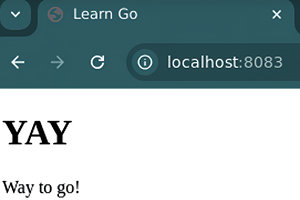
\includegraphics[width=0.66\textwidth]{figures/ch11/CH11_F03_Latour.png}
  \caption{浏览器中的页面}
  \label{fig:ch11-html-page}
\end{figure}

运行程序，享受一下 Web 诞生初期人人手写 HTML 的体验。图 \ref{fig:ch11-html-page} 展示了页面在浏览器里的样子。

看起来不错，不过代码里还有一个 \texttt{TODO} 需要照顾。


\subsubsection{使用正式的日志记录器}

现在要给服务器加一个像样的日志记录器。沿用第 10 章的思路：定义一个 \texttt{Logger} 类型，负责把日志写到指定输出，它只暴露 \texttt{Logf} 一个方法。日志记录器将成为服务器的依赖；服务器一侧则把依赖声明成接口，方便测试。

\begin{gocode}[title={代码清单 11.6 \texttt{log.go}：实现轻量日志记录器}]
// Logger is a lightweight logger.
type Logger struct {
    lgr *log.Logger #1
}

// New returns a logger that prints to the specified output.
func New(w io.Writer) *Logger {
    return &Logger{lgr: log.New(
        w, "", log.Ldate|log.Ltime)} #2
}

// Logf formats the message and sends it to the output.
func (l *Logger) Logf(format string, args ...any) {
    l.lgr.Printf(format, args...)
}
\end{gocode}

\begin{codeannotations}
\item 内部使用标准库的 \texttt{log} 包
\item 添加一组默认格式参数
\end{codeannotations}

接着把日志依赖加入服务器。这里不希望直接依赖 \texttt{log.Logger}：那会让测试变得痛苦。测试 \texttt{server} 包时，我们不想同时受 \texttt{log} 包具体实现的影响。更合适的做法，是在使用方声明一个本地接口，精确描述服务器需要日志记录器实现什么。

\begin{tipbox}{接受接口，返回具体类型}
“接受接口，返回具体类型”（accept interfaces, return types）是一条很实用的小原则，可以帮助你设计函数和方法签名。参数通常可以定义成所需的最小接口；返回值则往往没有必要使用接口，除非你确实想返回某种通用抽象。
\end{tipbox}

我们在 \path{log/logger.go} 中做出的选择，还受到 \texttt{testing.T} 的启发：它本来就实现了名为 \texttt{Logf} 的方法。于是测试时可以直接传入 \texttt{testing.T}，无须另建一个 \texttt{Logger} 变量。

\begin{gocode}[title={代码清单 11.7 \texttt{server.go}：接收日志记录器}]
type Logger interface { #1
    Logf(format string, args ...any)
}

type Server struct {
    lgr Logger #2
}

func New(lgr Logger) *Server { #3
    return &Server{lgr: lgr}
}
\end{gocode}

\begin{codeannotations}
\item 声明本地接口
\item 把日志记录器保存在服务器结构中
\item 通过参数注入日志记录器
\end{codeannotations}

最后更新 \texttt{main}：先构造日志记录器，再创建服务器时把它注入进去。以后无论是给习惯打卡，还是执行其他操作，后端发生了什么都能留下记录。服务器写往 \texttt{os.Stdout} 的内容不会发送给客户端，而会留在服务器“内部”，供开发者排查。

\subsubsection{对 HTML 做单元测试}

目前，根页面输出的是一份静态 HTML 文档。将来我们要用漂亮的界面管理习惯，为了保证它一直漂亮，现在就用 \texttt{httptest} 包把测试搭起来。

先检查调用 \texttt{index} 后一切顺利，并得到 \texttt{200 OK}。这里可以使用常见的 \texttt{github.com/stretchr/testify/assert} 与 \texttt{github.com/stretchr/testify/require} 包。

正如第 8 章所见，测试 HTTP 请求的输出需要 \texttt{httptest} 包提供的响应记录器。

\begin{gocode}[title={代码清单 11.8 \texttt{index\_test.go}：检查状态码}]
func TestServer_index(t *testing.T) {
    rr := httptest.NewRecorder() #1

    s := New(t) #2
    s.index(rr, nil) #3

    assert.Equal(t, http.StatusOK,
        rr.Result().StatusCode) #4
}
\end{gocode}

\begin{codeannotations}
\item 创建响应记录器
\item \texttt{testing.T} 实现了我们的 \texttt{Logger} 接口
\item 调用路径 \texttt{/} 的处理器
\item 检查状态码
\end{codeannotations}

要检查响应内容，可以准备一份真实 HTML 文件作为预期输出。它属于测试夹具（test fixture），因此应该放进 \texttt{testdata} 目录：

\begin{gocode}[]
expect, err := os.ReadFile("testdata/index.xhtml")
\end{gocode}

在测试语境中，这类文件常称为\emph{黄金文件}（golden file）。它保存生成内容应当遵循的“绝对真相”；有些项目习惯为它使用 \texttt{.golden} 后缀。

若直接比较两个字符串，结果可能会让你意外：制表符和换行方式造成的差异，也会被算作不相等，而测试其实不应该在意这些。为了让源码更易读而多加一个制表符，为什么就该让测试失败呢？

通常，比较整份输出并不是好主意；任何变化都可能让测试因为无关紧要的理由而坏掉。下面这种测试要求每一个空白字符都分毫不差。

\begin{gocode}[title={代码清单 11.9 \texttt{index\_test.go}：严格比较内容}]
expect, err := os.ReadFile("testdata/index.xhtml")
require.NoError(t, err)

assert.Equal(t, string(expect), rr.Body.String()) #1
\end{gocode}

\begin{codeannotations}
\item 严格的字符串比较
\end{codeannotations}

测试 HTML 有更好、也更曲折的办法。关键是先想清楚究竟要测试什么：我们并不是在测试 Go 的 \texttt{io.WriteString} 函数或 HTML 解析能力。前端框架已经深入思考过这类问题。这里暂时仍使用黄金文件，后面会找一些快捷办法，让这个版本足够令人满意。

运行测试。你也可以写一个错误路径测试，看看 \texttt{WriteString} 出错时会怎样——顺便想想，什么情况下它真的可能写失败。

现在，我们有了 HTML 输出，也有自动化测试监控它的变化。放心，我们再也不会把 HTML 写在 \texttt{.go} 文件里了（1987 年《日内瓦公约》以后，酷刑已经违法）。接下来就让模板登场救场。

\subsection{模板：显示一个变量}

格式化库 \texttt{fmt} 很擅长把一个变量按我们指定的格式输出；可一旦变量多起来，还要分散在不同的行上，它很快就会碰到极限。假设你要展示一家餐厅的菜单。每道菜可能有名称，也许还有便于员工和顾客沟通的编号、配料表、过敏原列表、是否适合素食者或纯素食者，以及价格。你当然可以用 \texttt{fmt.Sprintf} 来做，但那条语句超过 80 个字符的概率高得惊人。另一种办法是使用 \texttt{strings.Builder}；它稍好一些，却依旧折磨人。再想象一下：如果还要加入另一种语言的译文，或在某处补上热量数据，代码会变得多么难写、多么复杂。

当大片静态文本与少量动态值缠在一起时，模板就是一种合适的替代方案。本章会看到，模板能够非常清楚地表达结构化输出；你不必在调用 \texttt{Sprintf} 时数逗号，才能认出代码行里第四个 \texttt{\%s} 到底对应哪个值。

Go 自带两个模板库：\texttt{text/template} 和 \texttt{html/template}。两者接口相同，差别只在于 HTML 版本会自动转义对 HTML 敏感的字符，例如 \texttt{\&}、\texttt{<} 或 \texttt{é}。它还会保护生成文本免受代码注入：一个形如 \texttt{"</html>"} 的文本值不能提前结束浏览器正在渲染的页面，更恶意的 JavaScript 代码也不会因此被执行。

选择哪个库，应始终由功能需求决定。本章要渲染 HTML 文档，因此使用 HTML 模板。若不需要转义字符——只有 HTML 这类基于 XML 的语言才经常需要——标准的 \texttt{text/template} 通常足以覆盖需求。同样，用模板生成任何依赖标签的格式（例如 JSON），或依赖结构的格式（例如 YAML、CSV），都应该先问两个问题：能不能毫无防备地信任用户输入？模板收到一个“坏”值时，最糟会发生什么？

Go 模板把一段代码与一个模型绑定起来。模型以文本形式存在，通常从另一个文件加载；不过模板很短时，也可以直接定义成 \texttt{string} 变量。本章大部分模板都会放在外部文件中。

模板从来源加载并完成解析——也就是检查语法和文法——以后，就能在不同数据上执行并产生输出。Go 模板的核心概念是\emph{动作}（action）。模板引擎执行模板时，会依次应用其中的每一个动作。动作写在双重大括号之间：\texttt{\{\{...\}\}}。

可以把动作看成 \texttt{fmt.Printf} 调用中 \texttt{\%v} 的搭档：它是希望打印某个值的位置占位符。模板中不属于动作的内容会原样输出；动作则会在执行时作用于收到的值。要把值提供给模板动作，需要使用点号运算符 \texttt{.}。背景已经铺垫得够多了，现在开始写第一份模板。

\subsubsection{HTML 模板}

在真正充分使用 Go 模板之前，还有几步要走，不过现在至少可以先清理代码，把 HTML 从 Go 文件中抽出来，放进扩展名为 \texttt{.xhtml} 的真正 HTML 文件。这份文件就是模板。只要 IDE 能根据扩展名识别格式，它在这里也会更开心、更有用：既能协助排版，又能发现标记错误。完成第一个示例后，我们会继续搭建 HTTP 服务器。

第一项任务，是把一个变量传给模板，看看它如何渲染。就拿习惯数量来举例。把 HTML 字符串移入 \texttt{index.xhtml}，并使用动作 \texttt{\{\{.\}\}} 修改它——默认动作会打印当前变量，如下所示。这与在一段颇为复杂的字符串中间放一个 \texttt{\%v} 完全相同。

\begin{htmlcode}[title={代码清单 11.10 \texttt{index.xhtml}：输出变量}]
<!DOCTYPE html>
<html lang="en">
<head>
    <title>Learn Go</title>
</head>
<body>
<h1>Habits</h1>
<p>You have {{.}} habits to follow.</p> #1
</body>
</html>
\end{htmlcode}

\begin{codeannotations}
\item 在“have”和“habits”之间打印变量
\end{codeannotations}

\subsubsection{空格}

写成 \texttt{\{\{.\}\}} 并不算清楚。为了提高可读性，也可以写成带空格的 \texttt{\{\{ . \}\}}。两者严格等价；有人喜欢留空格，也有人不喜欢。你甚至可以混用 \texttt{\{\{.\}\}}、\texttt{\{\{ . \}\}}、\texttt{\{\{ .\}\}} 或 \texttt{\{\{. \}\}}，输出都一样。这里真正重要的是清楚、易读和前后一致。

不过，有时需要让一小段文本紧跟模板输出的值。假设要显示百分数，更合理的结果是 \texttt{17.5\%}，而不是 \texttt{17.5 \%}。模板可以写成 \texttt{\{\{.\}\}\%} 或 \texttt{\{\{ . \}\}\%}，但两种写法都可能让百分号不够显眼。为此，模板支持删除前后空白字符的功能。在动作任一侧加入减号（\texttt{-}），就会删除相应方向的空白——换行、制表符、不换行空格和普通空格都算，不过很奇怪，em space 与 en space 不算。使用 \texttt{-} 时，要让它紧贴花括号，同时与动作主体留出空格：不要写 \texttt{\{\{-.\}\}}，而应写 \texttt{\{\{- .\}\}}。还要记住，\texttt{-} 删除的是\emph{全部}空白，不只是在 \texttt{\{\{} 前刚刚输出的空格（或 \texttt{\}\}} 后的空格）；故意写入的制表符和换行也会一起消失。例如，下面几组写法分别会产生相同输出：

\begin{itemize}
  \item \texttt{\{\{ . -\}\} \%} 与 \texttt{\{\{.\}\}\%}；
  \item \texttt{\$\{\{ . \}\}} 与 \texttt{\$ \{\{- .\}\}}；
  \item \texttt{[ \{\{- . -\}\} ]}、\texttt{[\{\{.\}\}]}、\texttt{[ \{\{- .\}\}]} 以及其他变体。
\end{itemize}

第一份模板已经写好，接下来要让 Go 读取并填充它。代码清单 11.10 里“habits to follow”那个多余的复数 \texttt{s}，稍后也会处理——只有一个习惯时，它不该出现。

\subsubsection{在 Go 中使用模板}

首先，Go 要把文件读入变量。可以使用文件读取器，不过既然文件在不同运行之间不会变化，最合适的工具是 \texttt{go:embed} 指令：

\begin{gocode}[]
//go:embed index.xhtml
var indexPage string
\end{gocode}

这段语法表示：编译时把 \texttt{index.xhtml} 的内容放入这个变量。\texttt{embed} 只能用于包级变量。为了让编译器理解这条指令，需要导入 \texttt{embed} 包；但我们并不显式调用其中的函数或类型，所以要用下划线做“静默”导入：

\begin{gocode}[]
package server

import (
    _ "embed" // Allows us to load files
    // ...
)

//go:embed index.xhtml // Load the file contents to the indexPage variable.
var indexPage string
\end{gocode}

愿意的话，可以让单元测试也用这种方式获取预期值，而不再调用文件读取器。现在，用 \texttt{template.New} 创建模板并为它命名，然后调用 \texttt{Parse} 解析文件内容。\texttt{New} 接收我们想给模板起的名字，\texttt{Parse} 接收包含完整模板的字符串。模板为什么需要名字，到本章末尾就会揭晓；先说结论：模板之间可以通过注册名互相调用。

\begin{gocode}[]
template.New("index").Parse(indexPage)
\end{gocode}

终于可以让模板在某个值上执行了。调用返回错误的 \texttt{Execute} 方法即可。

\begin{gocode}[title={代码清单 11.11 \texttt{index.go}：输出变量}]
func (s *Server) index(w http.ResponseWriter, r *http.Request) {
    tpl, err := template.New("index").Parse(indexPage)
    if err != nil {
        // ...
    }

    err = tpl.Execute(w, 5) #1
    if err != nil {
        // ...
    }
}
\end{gocode}

\begin{codeannotations}
\item 传入一个习惯数量，例如 5
\end{codeannotations}

\begin{figure}[tbp]
  \centering
  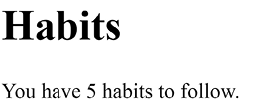
\includegraphics[width=0.58\textwidth]{figures/ch11/CH11_F04_Latour.png}
  \caption{变量在浏览器中的渲染结果}
  \label{fig:ch11-variable}
\end{figure}

务必在出错时返回内部错误，并记录原因。可以故意提供一份格式错误的模板来测试错误路径，例如少写一个花括号。图 \ref{fig:ch11-variable} 展示了代码清单 11.11 的结果。

更新测试输出、文档和所有必要内容，让代码经得住未来修改。下一步是调用后端服务——毕竟，谁会想要一张永远不显示实时数据的 Web 页面？

\subsection{添加 gRPC 客户端}

目前，HTTP 服务器什么也没连接。要返回“真实”数据，就得连到习惯服务器。在另一个终端中运行第 10 章的 \texttt{Habits} 服务，确定它在本机监听的端口并记下来，马上就会用到。本书示例使用 \texttt{8084}。可以借助集成测试，或用一组 \texttt{grpcurl} 命令，在服务数据库中加入几条虚拟习惯。

继续保持关注点分离这个好习惯。HTTP 服务器需要以下几个包：

\begin{description}
  \item[\texttt{habit}] 核心数据层，在这里定义可以在各包之间传递的数据结构；
  \item[\texttt{client}] 防腐层（anticorruption layer），把与后端通信所需的 gRPC 结构隔离在其内部，并简化调用；
  \item[\texttt{handlers}] 服务器在这里监听路由，并以 HTML 作出响应。
\end{description}

这些包都放在 \texttt{internal} 目录下。\texttt{main} 函数会依次把一个包注入另一个，最终组成一台功能完整的服务器。第一个 \texttt{habit} 包很容易起步：看看 gRPC 服务中的同名包，删掉不需要的内容即可。代码清单 11.12 展示了上一章定义的 \texttt{Habit} 结构；这里可以丢掉未通过 API 暴露的创建时间，转而加入本周已经打卡的次数。

\begin{gocode}[title={代码清单 11.12 \texttt{habit.go}：定义数据对象}]
// ID is the identifier of the Habit.
type ID string #1

// Name is a short string that represents the name of a Habit.
type Name string

// TickCount defines a number of ticks.
type TickCount uint

// Habit to track.
type Habit struct {
    ID              ID
    Name            Name
    WeeklyFrequency TickCount
    Ticks           TickCount #2
}
\end{gocode}

\begin{codeannotations}
\item 使用含义清楚的类型
\item 加入打卡次数
\end{codeannotations}

有了这块基石，服务器中的不同包就能互相传递习惯，而不必把各自的实现细节泄漏出去。

\subsubsection{后端客户端的结构}

回忆一下，上一章根据 Protobuf 定义生成的客户端拥有下面这个接口：

\begin{gocode}[]
type HabitsClient interface {
    CreateHabit(context.Context,
        *CreateHabitRequest,
        ...grpc.CallOption) (*CreateHabitResponse, error)
    ListHabits(context.Context,
        *ListHabitsRequest,
        ...grpc.CallOption) (*ListHabitsResponse, error)
    TickHabit(context.Context,
        *TickHabitRequest,
        ...grpc.CallOption) (*TickHabitResponse, error)
    GetHabitStatus(context.Context,
        *GetHabitStatusRequest,
        ...grpc.CallOption) (*GetHabitStatusResponse, error)
}
\end{gocode}

为了测试，我们希望能够模拟它。这意味着，\texttt{client} 包的 \texttt{New} 函数应该接收接口。恰好，所需接口已经生成，为什么不用呢？到本章结束时，这些方法全部都会用上。若只需要其中一部分，我们会在 \texttt{client} 包中另行声明一个本地接口。接下来先看怎样把第 10 章生成的接口导入当前模块。

\subsubsection{依赖本地包}

通过 \texttt{go mod init <module\_name>} 创建模块时，常见做法有两种。第一种很流行，主要用于命令行应用：直接给模块起一个名字。本书一直采用这种方式，本章 \texttt{go.mod} 的第一行就是 \texttt{learngo-pockets/templates}。另一种做法是使用模块的完整域名，例如 \texttt{k8s.io/kubernetes} 或 \texttt{github.com/grafana/grafana}。它主要用于库或准备分享的模块，不过应用程序当然也可以采用，上述示例正是如此。

现在遇到了一个问题：第 10 章的模块既没有发布，也没有公开，本章模块要怎样访问其中的文件？也就是说，怎样访问 \texttt{learngo-pockets/habits} 模块里的那份 gRPC 服务器定义？

若尝试使用标准命令添加依赖，会得到错误：

\begin{shellcode}[]
> go get learngo-pockets/habits
go: learngo-pockets/habits@v0.0.0-00010101000000-000000000000:
malformed module path "learngo-pockets/habits": missing dot in
first path element
\end{shellcode}

可以看到，Go 期望待导入模块的名称里出现一个点，也就是主机名与顶级域名之间的分隔符。也许可以尝试用相对路径导入本地 \texttt{.go} 文件，例如 \texttt{import "../habits/api"}。可这条路同样不会有好结局；随后解析导入时会报错：

\begin{shellcode}[]
> go mod tidy
../habits/api/: "../habits/api" is relative, but relative import
paths are not supported in module mode
\end{shellcode}

要解开这个难题，可以使用 \texttt{go mod edit -replace}，覆盖某个模块的版本或路径。它主要有两种用途：指定库应使用哪个版本、标签或分支；或者指向一个本地实现。语法如下：

\begin{shellcode}[]
> go mod edit -replace=old_module=new_module
\end{shellcode}

例如，假设我们把 \texttt{github.com/stretchr/testify} 的本地克隆保存在 \path{../stretchr/testify}（也可以使用绝对路径），就可以执行：

\begin{shellcode}[]
> go mod edit -replace=github.com/stretchr/testify=../stretchr/testify
\end{shellcode}

若要指定版本、分支或标签，只需追加 \texttt{@} 和相应引用：

\begin{shellcode}[]
> go mod edit -replace=github.com/moby/moby=github.com/moby/moby@dev
\end{shellcode}

当前情况是：要使用同一台机器上另一路径中的模块版本。必须提供模块路径，而不是包路径；按照本书的目录结构，命令如下：

\begin{shellcode}[]
> go mod edit -replace=learngo-pockets/habits=../10-habits/7_track
\end{shellcode}

若没有完成第 10 章，可以从本书代码仓库克隆对应实现，再用正确路径运行这条命令。

现在查看 \texttt{go.mod}，应该能看到一行——通常位于文件末尾——显示 \texttt{replace} 命令的效果：

\begin{plaincode}[]
replace learngo-pockets/habits => ../10-habits/7_track
\end{plaincode}

很好！现在可以导入 \texttt{learngo-pockets/habits} 模块中的 \texttt{api} 包，Go 也能找到这个本地包。不过要记住，这样会把依赖绑在一个本地文件路径上；把项目分享给同事时，十有八九会出问题。因此，几乎总是更好的做法，是以某个域名（例如 \texttt{github.com}）为前缀发布模块，让 Go 工具链能够从那里获取。

\subsubsection{实现 gRPC 客户端}

现在已经能访问后端服务定义了。请在 \texttt{internal/client} 包中创建新的客户端结构，只保留一个字段：我们不希望服务其他部分直接接触的 gRPC 客户端。

\begin{gocode}[title={代码清单 11.13 \texttt{client.go}：封装客户端}]
// HabitsClient is a wrapper around the gRPC client.
type HabitsClient struct {
    cli api.HabitsClient #1
}

func New(cli api.HabitsClient) *HabitsClient {
    return &HabitsClient{cli: cli} #2
}
\end{gocode}

\begin{codeannotations}
\item gRPC 客户端
\item 通过参数接收客户端并完成构造
\end{codeannotations}

HTML 文档要列出所有已登记的习惯及其状态，还要让用户点一下就能打卡。这并不是单一功能，总得找个起点。从获取全部已登记习惯开始最合理，因为之后还可以使用它们的 ID 执行其他操作。

给客户端添加 \texttt{ListHabits} 方法，用来取回已经登记的习惯，如代码清单 11.14 所示。六边形架构主张把代码聚合成彼此独立的包；按照这种做法，\texttt{proto} 工具链生成的类型不应该暴露到 \texttt{client} 包之外。这个包的 API 只应依赖本地 \texttt{habit} 包定义的领域类型。

\begin{gocode}[title={代码清单 11.14 \texttt{list.go}：客户端列出习惯}]
// ListHabits lists the habits available.
func (hc *HabitsClient) ListHabits(ctx context.Context,
    t time.Time) ([]habit.Habit, error) { #1
    resp, err := hc.cli.ListHabits(ctx,
        &api.ListHabitsRequest{}) #2
    if err != nil {
        return nil, err
    }

    list := make([]habit.Habit, len(resp.Habits))
    for i, h := range resp.Habits {
        list[i] = habit.Habit{ #3
            ID:              habit.ID(h.Id),
            Name:            habit.Name(h.Name),
            WeeklyFrequency: habit.TickCount(h.WeeklyFrequency),
        }
    }
    return list, nil
}
\end{gocode}

\begin{codeannotations}
\item 传入一个时间戳，用来计算打卡次数
\item 调用后端
\item 从 gRPC 类型转换成本地域类型
\end{codeannotations}

我们还需要知道：对于每项习惯，在传入时间戳所在的那一周一共打过多少次卡。表示时间时，使用可与 Protobuf 兼容的 \texttt{timestamppb} 包。通过下面的命令添加依赖：

\begin{shellcode}[]
> go get google.golang.org/protobuf/types/known/timestamppb
\end{shellcode}

那一周的打卡数可以获取，不过后端只支持逐项查询：需要调用 \texttt{GetHabitStatus} 端点。因此，循环内部还要再发一次请求。

\begin{gocode}[title={代码清单 11.15 \texttt{list.go}：获取打卡次数}]
import "google.golang.org/protobuf/types/known/timestamppb"

// ...

for i, h := range resp.Habits {
    status, err := hc.cli.GetHabitStatus(ctx, #1
        &api.GetHabitStatusRequest{
            HabitId:   h.Id,
            Timestamp: timestamppb.New(t),
        })
    if err != nil {
        return nil, err
    }

    list[i] = habit.Habit{
        ID:              habit.ID(h.Id),
        Name:            habit.Name(h.Name),
        WeeklyFrequency: habit.TickCount(h.WeeklyFrequency),
        Ticks:           habit.TickCount(status.TicksCount),
    }
}
\end{gocode}

\begin{codeannotations}
\item 获取每项习惯的状态
\end{codeannotations}

现在正好可以思考一下：后端 gRPC API 的 \texttt{ListHabits} 端点是否应该顺便返回打卡数？或者，批量接收习惯列表的 \texttt{GetHabitStatuses} 会不会更好？我们的设计理由是，过早优化经常会把力气花错地方。《计算机程序设计艺术》的作者 Donald Knuth 曾写道：

\begin{quote}
大约有 97\% 的时候，我们都应该忘掉微小的效率问题：过早优化是万恶之源；但也不应错过那关键 3\% 中的机会。
\end{quote}

用户很少会拥有多到足以产生几百次相似调用的习惯；真有那么多，也许分页比给后端增加复杂度更合适。若代码真的投入生产，而监控工具显示大量资源都花在获取状态上，并且因此拖慢应用，那么上述两种方案就值得研究了。

这里本可以再加一层逻辑，处理联系后端服务时的超时。由于这不是本章主题，而且第 10 章已经讲过，我们暂且盲目信任后端连接足够可靠。生产环境里可千万别这么做！

这部分测试只有三条路径：成功；获取列表时报错；获取状态时报错。来为它们编写测试——一个 mock 返回数据，另外两个让 mock 返回错误。和第 5 章一样，这里仍用 \texttt{minimock} 生成 mock。

注意：只期待一次调用时使用 \texttt{minimock} 的 \texttt{Expect}；需要根据输入返回多种响应时，则使用稍显啰唆的 \texttt{Set}。

\begin{gocode}[title={代码清单 11.16 \texttt{list\_test.go}：测试成功路径}]
package client_test

//go:generate minimock -i \
// learngo-pockets/habits/api.HabitsClient -s "_mock.go" #1

func TestListHabits(t *testing.T) {
    mockClient := mocks.NewHabitsClientMock(t) #2

    mockClient.ListHabitsMock.Expect( #3
        minimock.AnyContext, #4
        &api.ListHabitsRequest{}).
        Return(&api.ListHabitsResponse{
            Habits: // ...,
        }, nil) #5
    mockClient.GetHabitStatusMock.Set(getHabitMock)

    habitsClient := client.New(mockClient) #6
    habits, err := habitsClient.ListHabits(
        context.Background(), time.Now())

    require.NoError(t, err) #7
    expectedHabits := // ...
    assert.Equal(t, expectedHabits, habits)
}

func getHabitMock(_ context.Context,
    in *api.GetHabitStatusRequest,
    _ ...grpc.CallOption) (*api.GetHabitStatusResponse, error) {
    if in.HabitId == "ID1" {
        return &api.GetHabitStatusResponse{TicksCount: 3}, nil
    }
    // ...
    return nil, fmt.Errorf("unexpected ID")
}
\end{gocode}

\begin{codeannotations}
\item 根据外部接口生成 mock
\item 创建 mock 实例
\item 模拟返回若干习惯的调用
\item 此处接受任意上下文
\item 设置调用的返回值
\item 实例化客户端
\item 确认一切顺利
\end{codeannotations}

这里测试的是客户端公开函数的行为，因此没有必要把测试写成内部测试。正因为如此，测试文件使用 \texttt{client\_test} 包，并导入实现所在的 \texttt{learngo-pockets/templates/internal/client}。接下来试试错误路径；当列举习惯本身就失败时，完全不必模拟 \texttt{GetHabitStatus} 调用。

\begin{gocode}[title={代码清单 11.17 \texttt{list\_test.go}：列举习惯返回错误}]
func TestListHabits_error(t *testing.T) {
    sentinelErr := fmt.Errorf("list habits error") #1

    mockClient := mocks.NewHabitsClientMock(t)
    mockClient.ListHabitsMock.Expect(minimock.AnyContext,
        &api.ListHabitsRequest{}).Return(nil, sentinelErr)

    habitsClient := client.New(mockClient) #2
    habits, err := habitsClient.ListHabits(
        context.Background(), time.Now())

    require.ErrorIs(t, err, sentinelErr) #3
    assert.Nil(t, habits)
}
\end{gocode}

\begin{codeannotations}
\item 定义预期错误
\item 使用会返回错误的 mock 实例化客户端
\item 断言确实收到该错误
\end{codeannotations}

第三个测试覆盖其中一次 \texttt{GetHabitStatus} 调用失败的情况。\texttt{ListHabits} 的 mock 返回有效数据，但查询第二项状态时返回错误。有些 mock 工具允许对同一端点多次调用类似 \texttt{Expect(EndpointName, ExpectedParameters)} 的方法，\texttt{minimock} 不允许。我们需要改写 mock 的行为：调用 \texttt{Set}，传入一份可以按实际调用自行适配的伪实现。

\begin{gocode}[title={代码清单 11.18 \texttt{list\_test.go}：获取状态返回错误}]
func TestListHabits_statusError(t *testing.T) {
    now := time.Now()
    mockClient := mocks.NewHabitsClientMock(t)
    habitsClient := client.New(mockClient)

    mockResponse := &api.ListHabitsResponse{
        Habits: []*api.Habit{
            {Id: "ID1", Name: "..."},
            {Id: "ID2", Name: "..."},
        },
    }

    sentinelErr := status.Error(codes.Internal, "not after 10PM")
    mockClient.ListHabitsMock.
        Expect(minimock.AnyContext, &api.ListHabitsRequest{}).
        Return(mockResponse, nil) #1

    mockClient.GetHabitStatusMock.Set(
        func(ctx context.Context,
            in *api.GetHabitStatusRequest,
            opts ...grpc.CallOption) (
            *api.GetHabitStatusResponse, error) {
            switch {
            case in.HabitId == "ID1":
                return &api.GetHabitStatusResponse{}, nil #2
            case in.HabitId == "ID2":
                return nil, sentinelErr #3
            default:
                return nil, fmt.Errorf("unexpected call")
            }
        })

    habits, err := habitsClient.ListHabits(context.Background(), now)

    require.ErrorIs(t, err, sentinelErr) #4
    assert.Nil(t, habits)
}
\end{gocode}

\begin{codeannotations}
\item 设定 \texttt{ListHabits} 调用的输出
\item 第一次 \texttt{GetHabitStatus} 成功
\item 第二次 \texttt{GetHabitStatus} 失败
\item 整体结果是错误
\end{codeannotations}

到这里，客户端的 \texttt{ListHabits} 逻辑已经通过测试。要真正使用它，还需要由 \texttt{main} 函数构造服务器所需的依赖。

\subsubsection{依赖注入}

一边是正在编写的 HTTP 服务器，另一边是用来获取习惯的 gRPC 客户端。负责实例化两者并把它们连接起来的，是 \texttt{main} 函数；它会按需把依赖注入下层。\texttt{server} 包不应该直接使用 \texttt{proto} 工具生成的 API，而应声明属于自己的小接口，描述一个习惯客户端需要做什么——这通常就是 Go 的做法。

\texttt{main} 函数要创建 gRPC 客户端，再把它交给 HTTP 服务器，如代码清单 11.19 所示。这里按照第 10 章集成测试中的方式实例化 gRPC 客户端。通常，远程依赖的地址不会是 \texttt{localhost:8084}——除非你格外幸运。另一项服务的地址应当能通过配置文件、Kubernetes ConfigMap、Docker 网络设置，或运行平台采用的其他方式注入。

\begin{gocode}[title={代码清单 11.19 \texttt{main.go}：构造客户端}]
func main() {
    cli, err := newClient("localhost:8084") #1
    if err != nil {
        log.Fatalf("create client: %v", err) #2
    }

    srv := handlers.New(cli, logger.New(os.Stdout))
    // ...
}

// newClient creates a client to the habits service.
func newClient(serverAddress string) (*client.HabitsClient, error) {
    creds := grpc.WithTransportCredentials(insecure.NewCredentials())
    conn, err := grpc.Dial(serverAddress, creds) #3
    if err != nil {
        return nil, err
    }

    grpcCli := api.NewHabitsClient(conn)
    return client.New(grpcCli), nil
}
\end{gocode}

\begin{codeannotations}
\item 写入后端服务端口
\item 已经没有继续运行的意义
\item \texttt{DialOption} 很多；完整列表可查看 \texttt{go doc grpc.DialOption}
\end{codeannotations}

HTTP 服务器需要知道该怎样使用这个新参数。更新 \texttt{server} 包的 \texttt{New} 函数，并从服务器视角声明那个很小、很容易模拟的接口，如代码清单 11.20 所示。多亏了这层接口，现在应该很清楚：HTTP 服务器完全不知道底层获取习惯用的是 gRPC 客户端。

\begin{gocode}[title={代码清单 11.20 \texttt{server.go}：使用客户端依赖}]
// HabitsClient is the dependency towards the Habits client.
//go:generate minimock -s "_mock.go" -o "mocks" #1
type HabitsClient interface {
    ListHabits(ctx context.Context,
        t time.Time) ([]habit.Habit, error)
}

// Server serves all the HTML routes on this service.
type Server struct {
    client HabitsClient #2
    lgr    Logger
}

// New builds a new server.
func New(cli HabitsClient, lgr Logger) *Server { #3
    return &Server{
        client: cli,
        lgr:    lgr,
    }
}

// Router returns an HTTP handler that listens to all the proper paths.
func (s *Server) Router() http.Handler {
    // ...
}
\end{gocode}

\begin{codeannotations}
\item 为测试生成依赖的 mock
\item 在服务器结构中加入字段
\item 构造时要求传入该依赖
\end{codeannotations}

最后回到 \texttt{index} 方法。现在可以通过接收者 \texttt{s} 访问后端客户端，并调用它取得习惯。HTTP 服务器调用 gRPC 服务时，当然希望一切顺利；但若真出了错，应当给客户端显示一个好看的 \texttt{5xx}（服务器内部错误）消息，如下面的代码所示。加一个“重试”按钮会很酷，不过先保持简单，相信用户知道怎样刷新页面。

\begin{gocode}[title={代码清单 11.21 \texttt{index.go}：后端发生错误时}]
// index serves the root page of the app.
func (s *Server) index(w http.ResponseWriter, r *http.Request) {
    habits, err := s.client.ListHabits(r.Context(), time.Now()) #1
    if err != nil {
        s.lgr.Logf("error! %s", err.Error()) #2
        http.Error(w, "Error while fetching data",
            http.StatusInternalServerError) #3
        return
    }
    // ...
}
\end{gocode}

\begin{codeannotations}
\item 使用请求携带的上下文
\item 记录错误
\item 因为还没有向 \texttt{w} 写入内容，可以返回一条不暴露细节的错误
\end{codeannotations}

\begin{figure}[tbp]
  \centering
  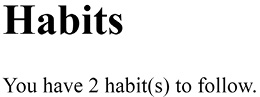
\includegraphics[width=0.55\textwidth]{figures/ch11/CH11_F05_Latour.jpg}
  \caption{使用真实习惯数量后的浏览器结果}
  \label{fig:ch11-real-count}
\end{figure}

当然，也可以更细致一些：在客户端包里检查 RPC 返回码，把它转换成命名错误，再在这里识别。眼下，无论后端返回哪一种错误码，都只意味着“内部出了问题”，所以这段实现已经够用。比如，将来给习惯服务器加入身份验证后，在适当情况下返回 \texttt{401} 就会更合理。

把模板 \texttt{Execute} 调用中硬编码的 \texttt{5} 替换成 \texttt{len(habits)}。图 \ref{fig:ch11-real-count} 展示了结果。

生成页面里的 \texttt{habits} 仍多了一个复数 \texttt{s}，而且每项习惯本身没有任何细节。该让列表登场，也该真正打开模板的力量了！

\section{模板的基本操作}

前面已经看到怎样在 HTML 模板中插入一个变量。本节继续介绍访问字段、表达条件等操作，并把一组习惯切片（\texttt{slice}）的内容展示出来。Go 模板本质上是一台引擎：它用传入的值更新一段字符串的内容。下面是一份独立的小例子。

\begin{gocode}[title={代码清单 11.22 使用模板遍历值}]
package main

import (
    "fmt"
    "os"
    "text/template" #1
)

func main() {
    tmpl := `{{ range . }}{{.}}, {{end}}` #2
    t, err := template.New("my_template").Parse(tmpl) #3
    if err != nil {
        fmt.Fprintln(os.Stderr, err)
        return
    }

    values := []string{"a", "b", "c"}
    err = t.Execute(os.Stdout, values) #4
    if err != nil {
        fmt.Fprintln(os.Stderr, err)
        return
    }
}
\end{gocode}

\begin{codeannotations}
\item 根据最终用途导入 \texttt{text/template} 或 \texttt{html/template}
\item 定义模板
\item 把定义解析成可执行模板
\item 在一组值上应用模板，并把结果写往某处
\end{codeannotations}

本节会帮助你理解模板，并说明从哪里开始使用它们。

\subsection{遍历一个切片}

模板不只会打印一个变量，它也有控制流语句。要遍历一组值，可以使用 \texttt{range} 动作。记住，在当前设置中，传给模板执行的是习惯切片，因此它由点号 \texttt{.} 表示：

\begin{htmlcode}[]
{{ range $index, $value := . }} <some html> {{ end }}
\end{htmlcode}

别忘了，\texttt{\{\{ end \}\}}（或 \texttt{\{\{end\}\}}）相当于 Go \texttt{for} 循环末尾的右花括号。输入值可以是切片、映射（\texttt{map}）、通道、数组，或任何 Go 知道怎样对其执行 \texttt{range} 的对象。写出 \texttt{\$index} 和 \texttt{\$value}，就会创建只在 \texttt{\{\{range\}\}...\{\{end\}\}} 块中可用的变量。比如，打印索引的动作是 \texttt{\{\{ \$index \}\}}。

另一种写法适用于模板中不需要索引变量的情况：使用 \texttt{\{\{ range . \}\} ... \{\{ end \}\}}，动作块内点号 \texttt{.} 的值会依次变成 切片中的各个元素。这个规则可能有些违背直觉：Go 代码若写 \texttt{for x := range values}，\texttt{x} 是 切片的索引或映射的键；模板里的 \texttt{\{\{ range . \}\}} 遍历的却是切片元素或映射的值。先用一组你喜欢的数字看看实际效果。

假如要在 Web 页面中以列表形式显示“\texttt{索引 : 数值}”，HTML 源码与刚才的语法不会相差太多。把下面这段加入 \texttt{index.xhtml} 的 \texttt{<body>} 区域。

\begin{htmlcode}[title={代码清单 11.23 \texttt{index.xhtml}：模板中的无序列表}]
<ul>
    {{ range $index, $value := . }} #1
    <li>{{ $index }} : {{ $value }}</li>
    {{ end }}
</ul>
\end{htmlcode}

\begin{codeannotations}
\item 循环遍历传入的数据
\end{codeannotations}

这里使用较完整的写法，因为我们要显示 \texttt{index}。随后只要把整数切片传给模板即可。

\begin{gocode}[title={代码清单 11.24 \texttt{index.go}：输出一个切片}]
values := []int{47, 52, 88, 18}

err = tpl.Execute(w, values) #1
if err != nil {
    // ...
}
\end{gocode}

\begin{codeannotations}
\item 把切片作为参数传给模板
\end{codeannotations}

\begin{figure}[tbp]
  \centering
  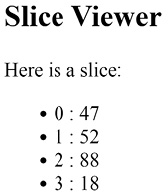
\includegraphics[width=0.48\textwidth]{figures/ch11/CH11_F06_Latour.jpg}
  \caption{浏览器中整数切片的渲染结果}
  \label{fig:ch11-int-slice}
\end{figure}

结果显得有点素，不过寥寥几行就已经得到一份能工作的演示。图 \ref{fig:ch11-int-slice} 展示了浏览器中的效果。

确认 \texttt{\{\{range\}\}} 与 \texttt{\{\{end\}\}} 能遍历整数切片后，回到习惯列表，尝试打印已经登记的各项目标。

\subsection{访问字段}

我们希望显示每项习惯的名称和每周目标频率。在无序列表（\texttt{ul}）中，每个列表项（\texttt{li}）都可以用粗体（\texttt{b}）显示名称，再显示每周次数，如图 \ref{fig:ch11-habit-list} 所示。有人认为粗体不该使用独立标签，而应是样式属性，应该把这里替换成 \texttt{span}。为了讲解清楚，我们姑且守旧一点；毕竟本章主题是 Go 模板，不是 HTML 语法。

\begin{figure}[tbp]
  \centering
  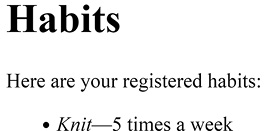
\includegraphics[width=0.58\textwidth]{figures/ch11/CH11_F07_Latour.jpg}
  \caption{浏览器中的习惯列表}
  \label{fig:ch11-habit-list}
\end{figure}

这个例子的静态 HTML 很直白：

\begin{htmlcode}[]
<ul>
  <li>
    <b>Knit</b> - 5 times a week
  </li>
</ul>
\end{htmlcode}

要得到同样结果，模板已经在遍历习惯。这里采用简写：\texttt{\{\{range .\}\}} 中的 \texttt{.} 表示习惯切片；进入范围以后，点号则表示当前正在遍历的那项习惯，如代码清单 11.25 所示。访问这一项的字段，只要在点号后写字段名。字段\emph{必须导出}！这意味着模板与代码库耦合得很紧：字段一旦改名或变成未导出，模板就再也打印不出它。

\begin{htmlcode}[title={代码清单 11.25 \texttt{index.xhtml}：访问字段}]
<ul>
    {{- range .}} #1
    <li>
        <b>{{ .Name }}</b> - {{ .WeeklyFrequency }}
        time(s) a week #2
    </li>
    {{- end}}
</ul>
\end{htmlcode}

\begin{codeannotations}
\item 这里的点号表示整个 \texttt{slice}
\item 这里的点号表示当前元素；访问习惯的 \texttt{Name} 与 \texttt{WeeklyFrequency}
\end{codeannotations}

执行模板时，把习惯 \texttt{slice} 交给它：

\begin{gocode}[]
err = tpl.Execute(w, habits)
\end{gocode}

所有习惯都看到了吗？测试是不是坏了？是不是正在和测试里的空白字符搏斗？记住，\texttt{\{\{-} 或 \texttt{-\}\}} 可以帮助删除多余的空格、换行和制表符。

现在已经可以自由尝试展示习惯的不同字段。你也许很想直接取得某个方法的输出——毕竟，方法不也和字段一样，是类型公开出来的吗？这里必须先给出一条警告：模板确实能调用方法，但有两个主要条件：

\begin{itemize}
  \item 方法必须是无参方法，也就是不接收显式参数；
  \item 方法必须返回一个值，或者返回两个值且第二个是错误。后一种情况下，模板会打印第一个返回值。
\end{itemize}

只要符合条件，就能在模板中不写括号地调用：\texttt{\{\{ .Method \}\}}。官方文档甚至指出，还可以把调用串起来，例如 \texttt{\{\{ .Field1.Method1.Field2.Method2 \}\}}。为了代码清楚，我们完全不推荐这样做。请不要这么写。稍后会看到，更好的办法是使用函数或专门的子模板。

在继续为用户增加功能之前，先解决“habit(s)”里那个括号中的小写 \texttt{s}。

\subsection{条件格式}

有些面板只想在特定条件下显示。好消息是，模板内部可以使用 \texttt{if} 模式。和 Go 一样，它有几种关键字：

\begin{htmlcode}[]
{{ if <condition> }}
{{ else if <condition> }}
{{ else }}
{{ end }}
\end{htmlcode}

这里的 \texttt{end} 与关闭 \texttt{range} 语句作用域时使用的是同一个关键字。

条件写法略有不同：比较操作在前，操作数在后。比较符号是严格定义的，例如 \texttt{lt} 表示“严格小于”，\texttt{ge} 表示“大于或等于”。表 \ref{tab:ch11-conditions} 列出更多 Go 模板条件。

\begin{table}[tbp]
\centering
\caption{Go 代码与模板条件的对应关系}
\label{tab:ch11-conditions}
\small
\begin{tabularx}{\textwidth}{@{}Y Y@{}}
\toprule
\textbf{Go 代码} & \textbf{Go 模板} \\
\midrule
\texttt{if h}（布尔值） & \texttt{\{\{ if . \}\}} \\
\texttt{if h != 0}（任意数值类型，包括 \texttt{rune}） & \texttt{\{\{ if . \}\}} \\
\texttt{if h != ""}（字符串） & \texttt{\{\{ if . \}\}} \\
\texttt{if len(h) != 0}（切片、映射、数组或字符串，不含通道） & \texttt{\{\{ if . \}\}} \\
\texttt{if h != nil}（接口、未初始化的切片、映射、通道或指针） & \texttt{\{\{ if . \}\}} \\
\texttt{if h < 3}（数值） & \texttt{\{\{ if lt . 3 \}\}} \\
\texttt{if h == "pockets"} & \texttt{\{\{ if eq . "pockets" \}\}} \\
\texttt{if h >= -8} & \texttt{\{\{ if ge . -8 \}\}} \\
\texttt{if h != 4} & \texttt{\{\{ if ne . 4 \}\}} \\
\texttt{if s.X < 40 \&\& !s.End} & \texttt{\{\{ if and (lt .X 40) (not .End) \}\}} \\
\bottomrule
\end{tabularx}
\end{table}

借助 \texttt{\{\{if\}\}} 动作，每周次数终于可以在只有一次时使用单数形式。注意这里用 \texttt{-} 删除多余空格：

\begin{htmlcode}[]
{{ .WeeklyFrequency }} time{{ if gt .WeeklyFrequency 1 -}}s{{- end }} a week
\end{htmlcode}

甚至可以使用 \texttt{once}、\texttt{twice} 这样更自然的词：

\begin{htmlcode}[]
{{ if eq .WeeklyFrequency 1 }}once
{{- else if eq .WeeklyFrequency 2 }}twice
{{- else }}{{ .WeeklyFrequency }} times
{{- end }} a week
\end{htmlcode}

对最终用户来说，结果不一定更容易读——这件事可以去问用户体验设计师——但它确实能工作，图 \ref{fig:ch11-frequencies} 展示了效果。这种复杂逻辑可以提取成函数，第 \ref{sec:ch11-template-functions} 节会介绍。

如今，页面已经能显示数据库中的真实数据。不过我们仍然只能读；身为用户，无法登记自己做过的活动，肯定会很沮丧！进入下一步之前别忘了测试。如果模拟的 \texttt{Habits} 服务调用已经返回了数据，只需要更新测试输出；也要确保错误路径都受到覆盖。

\begin{figure}[tbp]
  \centering
  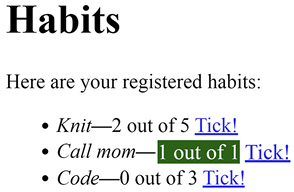
\includegraphics[width=0.75\textwidth]{figures/ch11/CH11_F08_Latour.jpg}
  \caption{习惯列表及各自的每周频率}
  \label{fig:ch11-frequencies}
\end{figure}

提交代码。现在该告诉系统：待办事项里有些事情已经完成了。

\section{向服务器发送一次打卡}

把待办事项从脑袋里挪到纸上，是个好办法；但只有把方框真正勾起来，一天才会显得卓有成效。认知研究指出，对于格外看重生产力的人，保留一张“已完成”清单有益健康，因为它能带来成就感。和始终盯着一长串“拖了这么久还没处理”的事情相比，这对大脑友好多了。

\subsection{操作之后该显示哪一页}

本章选择让全部逻辑发生在服务器端，而不是浏览器内部。这意味着，要向服务器发送信息或命令——例如“现在给 ID 为 987 的习惯打卡”——能要求用户浏览器做的唯一动作，就是前往另一个页面。另一种方案是使用 JavaScript 向 HTTP 服务器发请求，不过这里不采用它。

HTML 中的“HT”代表超文本（Hypertext），所以我们可以动用这门古老魔法：让一段文字把用户带到另一个页面。目标是实现一个 HTTP 端点，按给定 ID 为习惯打卡。目标 URL 为 \texttt{/tick/\{habitID\}}。先为列表中的每项习惯加上链接。

\begin{htmlcode}[title={代码清单 11.26 \texttt{index.xhtml}：为每项习惯添加打卡链接}]
<li>
    <!-- ... -->
    <a href="/tick/{{ .ID }}">Tick!</a> #1
</li>
\end{htmlcode}

\begin{codeannotations}
\item HTTP 链接
\end{codeannotations}

点击以后，浏览器会跳转到该链接，并尝试用 \texttt{GET} 取得页面。既然这是一项操作，按理说应该使用 \texttt{POST}；下一节再处理。眼下先用 \texttt{GET}，如代码清单 11.27 所示。把这条路由加入服务，避免经典的 \texttt{404}。前几章已经见过，Go 标准 \texttt{http} 包把花括号中的字符串理解为路径参数。

\begin{gocode}[title={代码清单 11.27 \texttt{server.go}：注册打卡端点路由}]
func (s *Server) Router() http.Handler {
    // ...
    r.HandleFunc(http.MethodGet+" "+"/tick/{habitID}", #1
        s.tick)
    return r
}
\end{gocode}

\begin{codeannotations}
\item 注册带有 \texttt{habitID} URL 参数的路由
\end{codeannotations}

现在要在服务器上实现新的 \texttt{tick} 方法。它的签名已经由 \texttt{http} 包规定：必须能作为 \texttt{http.HandlerFunc} 使用。第一步，通过 \texttt{http.Request} 的 \texttt{PathValue} 方法，从请求 URL 解析标识符。第二步是调用客户端，不过先把这部分留到最后。在新文件 \texttt{tick.go} 中编写端点。

\begin{gocode}[title={代码清单 11.28 \texttt{tick.go}：为习惯打卡}]
// tick adds a tick to the given habit.
func (s *Server) tick(w http.ResponseWriter, r *http.Request) {
    const habitIDPathValue = "habitID"

    id := r.PathValue(habitIDPathValue) #1
    if id == "" {
        http.Error(w, "missing the id of the habit",
            http.StatusNotFound)
        return
    }

    // TODO call the gRPC client
}
\end{gocode}

\begin{codeannotations}
\item 使用 URL 参数的名字
\end{codeannotations}

下一步要给用户一些反馈。可以写“干得漂亮，点这里回到主页”，但我们不想要求用户多点一次，从而加重可能存在的腕管综合征。另一种办法，是等后端 \texttt{Tick} 端点调用完毕，再悄悄显示主页：

\begin{gocode}[]
s.index(w, r)
\end{gocode}

这样确实能用，可以试试看。用户前往 \texttt{/tick/ID}，看到更新后的主页；可一旦刷新页面，就会再记一次打卡，这显然不合直觉。

好在，需要在向服务器发送命令后重定向的开发者不止我们。HTTP 状态码 \texttt{303}，其雅致名称是 \texttt{See Other}，仿佛就是为这件事准备的：

\begin{gocode}[]
http.Redirect(w, r, "/", http.StatusSeeOther)
\end{gocode}

这会告诉浏览器回到另一个页面，在本例中就是主页。此时，给主页路径定义常量的好处就体现出来了：重定向到名为 \texttt{indexPath} 的常量，比前例中神秘的 \texttt{"/"} 更清楚。

现在已经可以测试一部分逻辑：读取 \texttt{habitID}。照例需要一个 \texttt{ResponseRecorder}，还要用 \texttt{SetPathValue} 为请求设置 URL 参数。把测试写到 \path{handlers/tick_test.go}。

\begin{gocode}[title={代码清单 11.29 \texttt{tick\_test.go}：测试 URL 参数}]
func TestServer_Tick(t *testing.T) {
    rr := httptest.NewRecorder()

    req := httptest.NewRequest( #1
        http.MethodGet, "/tick/", nil)
    req.SetPathValue("habitID", "1234") #2

    s := New(nil, t)
    s.tick(rr, req)

    assert.Equal(t,
        http.StatusSeeOther, rr.Result().StatusCode) #3
    assert.Contains(t, rr.Body.String(), `<a href="/">`) #3
}
\end{gocode}

\begin{codeannotations}
\item 像往常一样创建请求
\item 提供 URL 参数
\item 验证状态码与重定向
\end{codeannotations}

这个测试并没有覆盖完整流程，而是直接提供一份已经准备好数据的请求。看起来有点像作弊，但这是单元测试，我们不想同时测试 \texttt{PathValue} 的逻辑，以及调用 \texttt{tick} 方法之前发生的事情。真想验证整条链路，就应该写集成测试：运行服务，并像真正的客户端那样调用它。这里选择保持在单元测试的范围内。这个端点已经像模像样，却还没有真正完成工作；接下来要调用 gRPC 客户端。

\subsection{把打卡发送给后端}

终于要把客户端接到后端 \texttt{Habits} 服务器了。沿用 \texttt{ListHabits} 的模式，在 \texttt{HabitsClient} 上编写 \texttt{TickHabit} 方法。它接收 \texttt{context.Context} 与习惯 ID，并可能返回错误；内部则隐藏对 gRPC 客户端的调用。后端 \texttt{TickHabit} 的响应为空，因此只保留返回的错误（若有）即可。

不过，后端请求还要求提供发生打卡的时间戳。我们怎样告诉客户端要处理哪一周？先在下一份代码里把当前时间写死，稍后在第 \ref{sec:ch11-multiple-values} 节再回来增加参数。

\begin{gocode}[title={代码清单 11.30 \texttt{tick.go}：调用后端打卡}]
// TickHabit adds a tick now.
func (hc *HabitsClient) TickHabit(ctx context.Context,
    id habit.ID) error {
    req := api.TickHabitRequest{
        HabitId:   string(id),
        Timestamp: timestamppb.Now(), #1
    }

    _, err := hc.cli.TickHabit(ctx, &req) #2
    return err
}
\end{gocode}

\begin{codeannotations}
\item 生成与 Protobuf 兼容的当前时间戳
\item 调用习惯服务
\end{codeannotations}

可以看到，如果 API 以后改变，后端开始返回有用的响应，就是这一层负责决定怎样处理、是否继续向外暴露。使用新方法之前，还要更新服务器侧的 \texttt{HabitsClient} 接口，如代码清单 11.31 所示。服务器对客户端层的依赖原本只暴露 \texttt{ListHabits}；把 \texttt{TickHabit} 加进去并重新生成 mock。最后，在服务器层的 \texttt{tick} 方法中调用客户端，用漂亮的 mock 写一份测试，运行并欣赏结果。现在不仅能显示登记过的习惯，还能点击页面记录进展了。

\begin{gocode}[title={代码清单 11.31 \texttt{server.go}：在接口中加入 \texttt{TickHabit}}]
//go:generate minimock -s "_mock.go" -o "mocks"
type HabitsClient interface {
    ListHabits(ctx context.Context,
        t time.Time) ([]habit.Habit, error)
    TickHabit(ctx context.Context, id habit.ID) error
}
\end{gocode}

把客户端 mock 加入单元测试，并检查它确实收到正确的 \texttt{Habit} ID。运行服务器，点击 \texttt{Tick!} 链接，计数器应该随之更新。虽然这已经很棒，我们仍可以通过视觉反馈改善体验，让现有数据更容易理解。

\subsection{添加颜色}

HTML 有一位能赐予它漂亮颜色的挚友：层叠样式表（Cascading Style Sheets，CSS）。之所以称为“层叠”，是因为容器属性会从父容器继承。省略前端理论，只说眼前需要的部分：可以为任意 HTML 标签添加类，再给这个类应用样式。列表项（或其他容器）的代码不会因此多出多少，浏览器里的渲染结果却会完全不同。

\begin{tipbox}{延伸阅读}
想进一步学习 CSS，可以阅读 Keith J. Grant 的 \emph{CSS in Depth}（Manning，2024，第 2 版）。
\end{tipbox}

为打卡次数已经达到每周目标的习惯创建一个名为 \texttt{done} 的 CSS 类，再给列表项添加 \texttt{class} 属性。判断目标是否完成时，使用模板中的 \texttt{\{\{ if ... \}\}}，比较打卡数与目标值。

注意：如果目标是每周写三次代码，而实际写了更多次，也仍然算完成；也就是说，大于或等于目标的次数都可以。

\begin{htmlcode}[]
<li class="{{ if ge .Ticks .WeeklyFrequency }}done{{end}}">
\end{htmlcode}

其实，这项逻辑更应该放在 Go 中，因为那样更容易测试。一个 \texttt{Habit} 变量应该能自己说明是否已经完成。编写并测试这个方法。记得模板只能访问导出方法。在 \texttt{habit} 上加入代码清单 11.32 所示的 \texttt{IsDone}，然后在模板中调用它，替换上一行代码。

\begin{htmlcode}[]
<li class="{{ if .IsDone }}done{{end}}">
\end{htmlcode}

\begin{gocode}[title={代码清单 11.32 \texttt{habit.go}：暴露习惯是否完成}]
// IsDone returns whether a habit has been fully completed.
func (h *Habit) IsDone() bool {
    return h.Ticks >= h.WeeklyFrequency
}
\end{gocode}

在 \texttt{<head>} 标签内部加入下面的样式代码，让差异显现出来。这里刻意保持最简，并不打算示范 CSS 应该怎样组织。

\begin{htmlcode}[]
<head>
<!-- ... -->
<style>
  .done {
    color: white;
    background-color: darkgreen;
  }
</style>
<!-- ... -->
</head>
\end{htmlcode}

尽管按照自己的口味更换颜色，也请考虑色觉障碍用户。重启服务器并检查结果：为一项习惯打够目标次数后，它的外观改变了吗？更新测试，确保它顺利通过，并覆盖所有相关情况。

\section{用表单创建习惯}

软件开发总是在努力把小步增量尽早交给用户，以便让产品与真实需求保持一致。更实际地说，小幅变更也能让产品更早部署、尽快产生收入。把一个想法变成现实——无论是一整款产品，还是单个功能——通常都从寻找最小可行产品（minimum viable product，MVP）开始：尽可能剔除功能，再根据用户反馈不断迭代。我们已经把“在指定日期打卡”推迟到了以后，但还有一个功能缺了就根本无法发布：创建习惯。

\subsection{HTML 表单}

要创建习惯，需要从用户那里取得名称、频率等值。为此，让用户填写一张表单，并提供一种把习惯“发送”给服务器、由服务器完成创建的方式。HTML 的 \texttt{form} 标签正是用来向服务器发送数据的。它可以拥有许多属性，本节只关注两个：\texttt{action} 决定数据发送到哪条路径，\texttt{method} 决定使用哪个 HTTP 动词。

\begin{htmlcode}[]
<form action="/create" method="post">
\end{htmlcode}

要创建习惯，\texttt{POST /create} 已经足够直白。若系统还要处理其他类型的实体，礼貌的做法是给路径加上 \texttt{habits} 前缀；这里保持简单。

\texttt{form} 元素内部还能包含若干各司其职的元素。当前只需要三种：让用户输入数据的 \texttt{input}、说明输入内容的 \texttt{label}，以及负责向服务器发起调用的 \texttt{button}。

从服务器角度看，只需为每个字段附上名字，用来区分它们。\texttt{input} 标签就是为此使用的：它表现为一块空白区域，用户可以在其中写入数据。但从用户角度看，还得显示一些文字，告诉他们各个输入框期待什么；这是 \texttt{label} 的职责。\texttt{label} 的 \texttt{for} 属性要与相应 \texttt{input} 的 \texttt{id} 一致。

屏幕阅读器等辅助视障人士使用的程序，会大量利用标签。更多信息可参阅 W3C 的 Web Accessibility Initiative（WAI）。最后，用户点击 \texttt{button} 后，表单数据就会发送给服务器。完整表单如下。

\begin{htmlcode}[title={代码清单 11.33 \texttt{index.xhtml}：创建习惯的表单}]
<form action="/create" method="post">
    <label for="habitName">Objective:</label> #1
    <input type="text" id="habitName" name="habitName">

    <label for="habitFrequency">Weekly frequency:</label> #2
    <input type="number" id="habitFrequency" name="habitFrequency">

    <button>Create</button>
</form>
\end{htmlcode}

\begin{codeannotations}
\item \texttt{habitName} 标签的 \texttt{for} 与输入框的 \texttt{id} 相匹配
\item \texttt{habitFrequency} 标签的 \texttt{for} 与输入框的 \texttt{id} 相匹配
\end{codeannotations}

在浏览器中检查结果；愿意的话，也可以加上漂亮样式。图 \ref{fig:ch11-form} 展示了没有加样式的版本。

\begin{figure}[tbp]
  \centering
  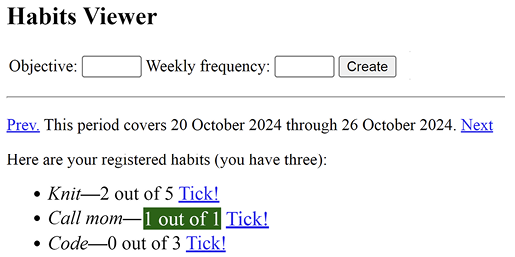
\includegraphics[width=0.82\textwidth]{figures/ch11/CH11_F09_Latour.png}
  \caption{浏览器中的习惯创建表单}
  \label{fig:ch11-form}
\end{figure}

\subsection{读取表单值}

点击按钮后，数据会发送到前面定义的 \texttt{/create} 路由；现在要让服务器监听它。为了实现完整调用链，还需要调用后端的 \texttt{CreateHabit} 端点。先从 \path{internal/client/create.go} 开始。实现很直接：接收一项习惯的定义，把它转换成 Protobuf 表示，再调用后端端点。使用模拟的 gRPC 客户端测试它，策略与测试 \texttt{TickHabit} 相同。

接着在服务器上添加一个与 \texttt{tick} 类似的处理器。数据可以通过 \texttt{http.Request} 的 \texttt{FormValue} 方法取得，但它只返回字符串。使用 \texttt{strconv} 包，把目标频率解析成整数。

\begin{gocode}[title={代码清单 11.34 \texttt{create.go}：解析表单值}]
// create takes form values and creates a Habit from them,
// then redirects to index.
func (s *Server) create(w http.ResponseWriter, r *http.Request) {
    habitName := r.FormValue("habitName") #1
    weeklyFreq, err := strconv.Atoi(
        r.FormValue("habitFrequency")) #2
    if err != nil {
        // ...
    }

    // call client

    // redirect to index
    http.Redirect(w, r, "/", http.StatusSeeOther) #3
}
\end{gocode}

\begin{codeannotations}
\item 读取字符串
\item 读取整数
\item 创建新习惯以后刷新页面
\end{codeannotations}

最后更新路由器，注册新的 \texttt{POST} 端点：

\begin{gocode}[]
r.HandleFunc(http.MethodPost+" "+"/create", s.create)
\end{gocode}

新习惯的字段应该由谁验证？HTTP 服务器吗？毕竟尽早检查可以省掉无意义的网络调用。还是只由后端负责？毕竟后端才知道怎样的名称算“有效习惯名称”。这里决定不把完整业务验证放在前端。不过，这也提醒我们：HTTP 层仍需要一道安全网，保护后端免受恶意攻击。例如，可以先确认每周频率具有实际意义，也许限定在 1 到 100；同样，习惯名称可以要求长度在 1 到 200 个 rune 之间。

目前，用户输入无效数据时，还没有办法弹出窗口解释问题。服务器仍然把错误记录到 \texttt{os.Stdout}。本章主题毕竟是模板，接下来继续探索它们还能做什么。

\section{更多模板妙用}

我们已经见过模板中最常见的动作，以及它们的用法。Go 模板还有几种值得掌握的使用方式。

\subsection{向模板传递多个对象}
\label{sec:ch11-multiple-values}

执行模板时，习惯列表并不是唯一想传入的数据。这款产品姑且说是以“周”为单位设计的，可页面既没有显示日期，也无法在过去和未来的周之间导航。

先看看怎样显示一周的起止日期。约束在于：手里只有一份模板文档，也就是这张 HTML 页面，却希望向它传入多个值，而不只是当前的习惯列表。先决定页面要显示什么，再寻找实现办法。

\subsubsection{格式化的周类型}

若把时间戳直接传给模板并原样打印到页面，对用户很不友好。我们希望显示类似“6 月 30 日至 7 月 6 日这一周”的内容。为了简化代码，先规定每周从星期日开始。原因是 \texttt{time.Weekday} 的零值就是 \texttt{time.Sunday}；若改用星期一或星期六——另外两种常见的一周起点——或者马尔代夫采用的星期五，乃至任何其他日期，都要多做一点算术。

可以根据一个时间戳构造类型，再暴露两个方法：返回包含该时间戳那一周的 \texttt{Start} 与 \texttt{End}，如代码清单 11.35 所示。这个类型可以放在 \texttt{internal/habit} 包中，与全部业务类型待在一起——眼下另一个业务类型只有 \texttt{Habit}。

\begin{gocode}[title={代码清单 11.35 \texttt{week.go}：API}]
// FormattedWeek defines the start and end of a week, and formats them.
// Start to end will be from Sunday 00:00 to Saturday 23:59,
// rounded to the minute.
type FormattedWeek struct{} #1

// NewFormattedWeek builds an immutable week from one moment inside it.
func NewFormattedWeek(include time.Time) FormattedWeek #2

// Start returns the formatted first day of the week.
func (w FormattedWeek) Start() string #3

// End returns the formatted last day of the week.
func (w FormattedWeek) End() string #3
\end{gocode}

\begin{codeannotations}
\item 导出的类型
\item 根据给定时间构造
\item 只返回字符串的方法可以在模板中调用
\end{codeannotations}

这里有两个选择：保留传入时间戳，等需要时再计算一周的开始与结束；或者在 \texttt{NewFormattedWeek} 中预先计算起止时间，之后直接返回。后者会促使我们创建一个不可变类型；处理本例这类值对象时，这通常是好事。

在构造 \texttt{FormattedWeek} 实例时算出一周起止时间戳，并将它们保存在字段中。先从周内的那个时间得到当天零点——日期相同，时间是午夜——然后减去它在一周中的索引：星期日为 0，星期一为 1，依此类推。按天增减日期时使用 \texttt{AddDate}。这个方法允许在 \texttt{time.Time} 上增加或减少年、月、日，并替我们处理手写起来很痛苦的情形，例如闰年和冬令时／夏令时切换。还要记住，月份调整会经过日期规范化；因此在普通年份里，1 月 31 日加一个月可能得到 3 月 3 日，这也许会令人意外。\texttt{AddDate} 很实用，因为参数可以为负数，既能走向未来，也能回到过去。

\begin{gocode}[]
start := startOfDay(include).AddDate(0, 0, -int(include.Weekday()))
\end{gocode}

从这里再加七天、减一分钟，就得到本周结束时刻。如果连 1 毫秒都不减，结果会落在下一周星期日清晨，格式化出来就不是我们想要的日期。这里减去整整一分钟，是为了便于调试和测试；只要页面完全不显示时间、只显示日期，甚至可以减去一天。这也覆盖了不常见的闰秒问题。减一分钟要使用 \texttt{Add}。为什么同一种增减操作要分别用 \texttt{Add} 和 \texttt{AddDate}？因为两者的适用范围其实不同：短于一天的时长适合用 \texttt{Add}，超过一天的日历变化适合用 \texttt{AddDate}。代码清单 11.36 展示了 \texttt{NewFormattedWeek} 的实现。

\begin{gocode}[title={代码清单 11.36 \texttt{week.go}：构造格式化的一周}]
// FormattedWeek defines ...
type FormattedWeek struct {
    start, end time.Time #1
    layout     string
}

// NewFormattedWeek builds ...
func NewFormattedWeek(include time.Time, layout string) FormattedWeek {
    start := startOfDay(include).
        AddDate(0, 0, -int(include.Weekday())) #2
    return FormattedWeek{
        start:  start,
        end:    start.AddDate(0, 0, 7).
            Add(-1 * time.Minute), #3
        layout: layout,
    }
}

// startOfDay returns the same date as given, at midnight.
func startOfDay(t time.Time) time.Time {
    year, month, day := t.Date()
    return time.Date(year, month, day,
        0, 0, 0, 0, t.Location())
}
\end{gocode}

\begin{codeannotations}
\item 保存已经算出的时间戳
\item 计算包含参数时间的那一周起点
\item 计算一周终点
\end{codeannotations}

这类逻辑通常需要严格的单元测试：测试跨月、跨年的情况；输入位于星期日、星期一和星期六的情况；非 UTC 时区、夏令时切换期间，等等。

最后，还需要把两个时间戳格式化成人类能读懂的样子。\texttt{time} 包提供了相应函数，它接收一条布局字符串，例如 \texttt{"02 January 2006"}。Go 必须看到这种特定参考时间格式，才能理解布局。

可以把这个字符串硬编码成包常量，但决定内容怎样显示，真的是 \texttt{habit} 包的职责吗？理想情况下，布局参数应该传给 \texttt{Start} 和 \texttt{End} 方法。不过，为了先展示怎样在模板中调用无参方法，而不引入参数的复杂性，这里让“周”本身就是格式化过的——结构名也因此叫 \texttt{FormattedWeek}——把布局传给 \texttt{NewFormattedWeek} 并保存在字段中。于是两个方法的实现都很直接。

\begin{gocode}[title={代码清单 11.37 \texttt{Start} 与 \texttt{End} 方法}]
// Start returns the formatted first day of the week.
func (w FormattedWeek) Start() string {
    return w.start.Format(w.layout) #1
}

// End returns the formatted last day of the week.
func (w FormattedWeek) End() string {
    return w.end.Format(w.layout) #1
}
\end{gocode}

\begin{codeannotations}
\item 使用 \texttt{layout} 字段格式化时间
\end{codeannotations}

现在只剩一件事：相应更新 \texttt{NewFormattedWeek}。

\begin{tipbox}{支线任务 11.1}
把星期一或星期六设为一周的第一天，并相应更新测试。本书作者来自欧洲，因此仓库中的解答选择星期一；它放在另一个构建标签下，可参见 \url{https://mng.bz/OBzR}。
\end{tipbox}

\subsubsection{多个模板参数}

回到主页，先构造准备传给模板的一周：

\begin{gocode}[]
week := habit.NewFormattedWeek(time.Now(), "02 January 2006")
\end{gocode}

模板的 \texttt{Execute} 方法只能接收一个参数，而习惯列表已经占了这个位置。怎样再传时间戳之类的值？可以临时声明一个同时包含习惯列表和日期的结构，但用起来可能很啰唆。一张简单的映射（\texttt{map}）就能完成任务，如代码清单 11.38 所示。模板会把整张映射当作点号，再像访问字段一样用键访问其中的值。

\begin{gocode}[title={代码清单 11.38 \texttt{index.go}：传入更多数据}]
err = tpl.Execute(w, map[string]interface{}{
    "Habits": habits, #1
    "Date":   week,
})
if err != nil {
    // ...
}
\end{gocode}

\begin{codeannotations}
\item 模板可以通过 \texttt{.Habits} 访问习惯列表
\end{codeannotations}

在 HTML 中加一行显示日期。在 Go 模板里，调用方法看起来和访问字段相似：

\begin{htmlcode}[]
<p>This period covers {{.Date.Start}} -> {{.Date.End}}.</p>
\end{htmlcode}

你也许已经注意到，这一行只处理 \texttt{Date}。若它是 Go 代码，可以写一个接收 \texttt{Date}、返回起止日期的函数，把重复前缀提取掉。模板虽然也能声明变量来改善可读性，我们却不推荐，因为变量作用域过于宽松。更好的办法是使用 \texttt{with} 动作，把模板的视野限制在 \texttt{.Date} 字段内：

\begin{htmlcode}[]
{{with .Date}}<p>This period covers {{.Start}} -> {{.End}}.</p>{{end}}
\end{htmlcode}

在 \texttt{\{\{ with \}\} ... \{\{ end \}\}} 块内部，这种语法会把点号的“局部值”设为 \texttt{.Date}。当然，给模板传入多个参数后，习惯切片已经从 \texttt{.} 改名为 \texttt{.Habits}，因此 \texttt{\{\{range\}\}} 区域也要相应修改。甚至可以给整个列表块再包一层条件：切片为空时，根本不显示列表。

\begin{htmlcode}[title={代码清单 11.39 \texttt{index.xhtml}：隐藏空列表}]
{{- if .Habits }} #1
<!-- titles and nice displays -->
    <ul>
        {{- range .Habits }}
        <li>
            <!-- ... -->
        </li>
        {{- end }}
    </ul>
{{- end }}
\end{htmlcode}

\begin{codeannotations}
\item 使用 \texttt{-} 会从生成文档中删除这一空行
\end{codeannotations}

更新测试，并加入习惯切片为空的测试用例。图 \ref{fig:ch11-week-details} 展示了浏览器结果。

\begin{figure}[tbp]
  \centering
  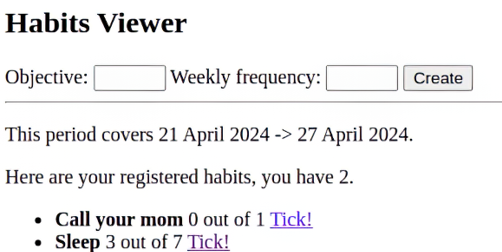
\includegraphics[width=0.88\textwidth]{figures/ch11/CH11_F10_Latour.png}
  \caption{浏览器中显示的一周详情}
  \label{fig:ch11-week-details}
\end{figure}

你看出为什么当前测试不可能一直稳定了吗？我们仍然用 \texttt{time.Now()} 作为这一周的输入。到了下周，测试就会坏掉。

\begin{tipbox}{支线任务 11.2}
既然已经能查看当前日期对应的习惯状态，不妨也看看前几周，并提前浏览后几周。可以按下面步骤自己实现：
\begin{enumerate}
  \item 在 HTML 中加入导航链接，并在格式化周类型上实现 \texttt{Previous} 与 \texttt{Next}：
\begin{htmlcode}[]
<a href="/?week={{ .Date.Previous }}">Prev.</a>
\end{htmlcode}
  \item 把时间作为查询参数传给主页；若参数不存在，就默认使用 \texttt{time.Now()}。路径参数是必填的，查询参数则不是。使用 \texttt{r.URL.Query().Get("week")} 从 URL 查询中取值。
  \item 更新客户端调用，把想查询的习惯周时间戳传进去。
  \item 给单元测试请求添加查询参数，并更新预期输出。
  \item 是否应该允许给过去的日期打卡？由你决定。界面应怎样表达？打卡后的重定向还会回到刚才那周吗，还是跳回当前周？怎样修复？
  \item 是否应该允许导航到未来？这有意义吗？怎样阻止用户进入未来周？只隐藏“下一周”按钮并不够——用户仍可能直接把未来时间戳作为查询参数传入。
\end{enumerate}
\end{tipbox}

\subsection{调用函数}
\label{sec:ch11-template-functions}

前面已经看到，模板引擎能访问值；它还能做得更多——模板可以运行函数。从某个角度看，\texttt{range} 和 \texttt{if} 之类的动作本身就很像函数，例如 \texttt{\{\{ range . \}\}} 与 \texttt{\{\{ if . \}\}}；我们也已经见过 \texttt{\{\{ len . \}\}}。你还可以在 Go 中编写自己的函数，再从模板调用。

\subsubsection{在模板中注册新函数}

目前，页面只显示习惯已经打卡多少次。这还不够有趣。Web 页面应该令人愉悦、色彩丰富，让访客愿意回来。来加一点这样的效果。

例如，可以按照本周目标已经完成的比例，为每项习惯显示不同颜色。编写一个函数计算进度，再针对不同阈值返回标签，如代码清单 11.40 所示。这个标签可以直接作为 CSS 类名，因此用字符串表示。它将替代之前的 \texttt{done} 类。

\begin{gocode}[title={代码清单 11.40 \texttt{index.go}：为进度生成标签}]
func statusCSSClass(h *habit.Habit) string {
    prog := float32(h.Ticks) /
        float32(h.WeeklyFrequency) #1
    switch {
    case prog == 0:
        return "not_started"
    case prog < 0.5:
        return "started"
    case prog < 1:
        return "good_progress"
    default: #2
        return "completed"
    }
}
\end{gocode}

\begin{codeannotations}
\item 计算完成比例
\item 已达到 1；若打卡数超过目标，也可能大于 1
\end{codeannotations}

要从模板调用这个函数，创建模板时必须通过 \texttt{Funcs} 方法先完成注册，如代码清单 11.41 所示。\texttt{Funcs} 接收一张函数映射：键是函数在模板中出现的名称，例如 \texttt{\{\{ myFunc . \}\}}；值则是真正要调用的 Go 函数。

\begin{gocode}[title={代码清单 11.41 \texttt{index.go}：向模板提供函数}]
tpl, err := template.New("index").
    Funcs(template.FuncMap{
        "statusCSSClass": statusCSSClass, #1
    }).
    Parse(indexPage)
if err != nil {
    // ...
}
\end{gocode}

\begin{codeannotations}
\item 把模板中的函数名映射到 Go 函数
\end{codeannotations}

现在，模板可以使用函数标识符，并把习惯作为参数传入。在 \texttt{\{\{ range .Habits \}\}} 循环内部，当前习惯由点号表示，因此可以像下面这样取得 CSS 类。

\begin{htmlcode}[title={代码清单 11.42 \texttt{index.xhtml}：使用函数}]
<style> #1
    li.habit.completed {
        background: #afa;
    }
    li.habit.good_progress {
        background: #ffa;
    }
    /* ... */
</style>
<!-- ... -->
<ul>
    {{- range .Habits }}
    <li class="habit {{ statusCSSClass . }}"> #2
        <b>{{.Name}}</b>
        <!-- ... -->
    </li>
    {{- end }}
</ul>
\end{htmlcode}

\begin{codeannotations}
\item 在 \texttt{<head>} 区域声明样式
\item 调用函数
\end{codeannotations}

运行程序，效果如何？当然可以自由更换颜色。别忘了补全 CSS，让它支持所有标签。为函数写单元测试，再更新 \texttt{index} 的测试。

\subsubsection{管道}

Go 模板支持\emph{管道}（pipeline）。当一个函数的输出要作为下一个函数的输入时，就适合使用它。Unix 用户会立刻认出这套语法，因为完全一样：\texttt{\{\{ func1 . | func2 \}\}} 与把 \texttt{func1(.)} 的结果传给 \texttt{func2} 等价，也就是通常写作 \texttt{func2(func1(.))} 的调用。管道中 \texttt{|} 的数量没有上限。

来看一个本章项目之外的例子。假设要打印一组 URL 中出现的主机名，并把输出统一规范成小写。首先需要一份 Go 函数，从 URL 中提取主机名；\texttt{net/url} 包可以完成这件事。

\begin{gocode}[title={代码清单 11.43 管道：从 URL 提取域名}]
func extractDomainName(rawURL string) string {
    u, err := url.Parse(rawURL)
    if err != nil {
        return "" #1
    }

    return u.Hostname()
}
\end{gocode}

\begin{codeannotations}
\item 传给模板的错误在这里不会得到真正处理
\end{codeannotations}

现在，把函数注册到这个小项目使用的模板里。因为还要把整条字符串转成小写，也一并注册 \texttt{strings.ToLower}。你也许会问：为什么不直接在 \texttt{extractDomainName} 内调用 \texttt{strings.ToLower}，非得费事注册两个函数？因为这个例子正要展示怎样用管道组合功能。模板可以这样构造：

\begin{gocode}[title={代码清单 11.44 注册管道中的全部函数}]
tmpl, err := template.New("domains").
    Funcs(template.FuncMap{
        "lower":             strings.ToLower,
        "extractDomainName": extractDomainName,
    }).
    Parse(`{{range .}}{{extractDomainName . | lower | println}}{{end}}`)
\end{gocode}

这里额外加了 \texttt{println}，让每个主机名独占一行；默认动作只会打印值，不会自动换行。把下面的切片传给模板：

\begin{gocode}[]
[]string{"http://google.com", "https://www.wikipedia.fr", "http://UN.org"}
\end{gocode}

会得到：

\begin{plaincode}[]
google.com
wikipedia.fr
un.org
\end{plaincode}

说到管道，\texttt{\{\{ . | len \}\}} 与 \texttt{\{\{ len . \}\}} 完全等价，都会打印值的长度。前一种写法更强调“正在操作哪个值”，后一种则更强调“使用哪个函数”。两种语法都有效，结果相同；开发者应根据具体场景选择更合适的一种。

\subsection{使用 define 声明模板函数}

本章最后要看的动作，是直接把“函数”写成模板动作，而不是在 Go 中通过 \texttt{Funcs()} 提供。它带来一个值得注意的结果：如果程序只负责加载和执行模板，那么只要更新它加载的模板文件，就可能改变程序行为。这在许多层面都很危险——必须跟踪当前使用的模板，必须保证模板始终正确，等等——但有时也会成为有趣的功能。

看看当前的 HTML 模板。我们用 \texttt{\{\{- range .Habits \}\}} 遍历习惯，走到相应的 \texttt{\{\{- end \}\}} 之前有五行代码。这五行唯一完成的事情，就是把一个结构转换成漂亮的列表项。它很适合提取成函数，顺便让代码更清楚。

这里定义一份新模板，职责是把习惯格式化成它的 HTML 表示。先在 HTML 文件中声明它。也可以把定义塞进整张页面所在的文件，不过那样很难找到一个不会让 HTML 骨架尖叫的位置。简单起见，放进另一份文件，如代码清单 11.45 所示。既然模板文件开始多于一个，不妨把 \texttt{index.xhtml} 移到新目录 \path{internal/handlers/templates}。再在同一目录中创建负责把习惯转换成 HTML 列表项的 \texttt{habititem.xhtml}。

声明模板的语法很短：使用 \texttt{\{\{ define "templateName" \}\} ... \{\{ end \}\}}。把原先 \texttt{\{\{range\}\}} 循环内部的内容从 \texttt{index.xhtml} 移到这里。

\begin{htmlcode}[title={代码清单 11.45 \texttt{habititem.xhtml}：在另一文件中声明模板}]
{{- define "habitItem"}}
        <li class="habit {{ statusCSSClass . }}">
            <b>{{.Name}}</b>
            <span class="{{ if ge .Ticks .WeeklyFrequency -}}
                done{{- end -}}">{{ progress . }}</span>
            <a href="/tick/{{ .ID }}">Tick!</a>
        </li>
{{- end }}
\end{htmlcode}

此处需要解释几项格式细节。可以看到，\texttt{\{\{- define \}\}} 与 \texttt{\{\{- end\}\}} 都以 \texttt{-} 开头，用来忽略它们之前的空白，包括前面的换行符 \texttt{\textbackslash n}。也可以反过来删除后面的换行，写成 \texttt{\{\{ define -\}\}} 与 \texttt{\{\{ end -\}\}}，甚至两边都加 \texttt{-}。但那样有个副作用：\texttt{-} 会删掉后续全部空白，包括缩进。浏览器渲染 HTML 时不会因此损坏，生成的源代码看起来却会很糟。这里还有另一点很重要：文件内容必须适当缩进。Go 模板没有提供专门的缩进函数；大量依赖 Go 模板处理 YAML 的 Helm 倒是提供了，所以 Helm 文件里经常能看到以 \texttt{| indent 4 \}\}} 结尾的动作。

现在更新 \texttt{index.xhtml}，调用新模板：把刚才复制出去的区域替换为动作 \texttt{\{\{ template "habitItem" . \}\}}。它会用当前点号值调用另一份模板；此时，点号正在遍历习惯。有时调用会省略最后的点号，写成 \texttt{\{\{ template "habitItem" \}\}}，因为点号是默认参数。这里仍然明确写出它。

\begin{htmlcode}[]
{{- range .Habits }}
    {{- template "habitItem" . }}
{{- end }}
\end{htmlcode}

我们再次选择缩进动作，以便阅读；不过请注意，调用 \texttt{"habitItem"} 前面的缩进，会被模板定义开头 \texttt{\{\{- define} 中的减号删掉。

文件移到新目录后，加载方式也要调整。\texttt{index.xhtml} 中并没有显式导入 \path{habititem.xhtml}，它怎样引用另一文件里的模板？以前只嵌入一份模板文件，现在是否要嵌入多份？列到多长以后才显得荒唐？本书不替你规定上限，不过我们认为超过一份就已经够多了，因此不逐一嵌入文件。既然两份模板都放在同一目录，可以直接嵌入整个目录的内容！编译时，它们都会被加载到内存。代码清单 11.46 展示了 \texttt{index.go} 的变化。

\begin{gocode}[title={代码清单 11.46 \texttt{index.go}：嵌入一个目录的内容}]
//go:embed templates/*.xhtml #1
var templates embed.FS

// ...
tpl, err := template.New("index").Funcs(template.FuncMap{
    "statusCSSClass": statusCSSClass,
    "progress":       progress,
}).ParseFS(templates, "templates/*.xhtml") #2
\end{gocode}

\begin{codeannotations}
\item 收录模板目录中扩展名为 \texttt{.xhtml} 的全部文件
\item 解析模板目录中扩展名为 \texttt{.xhtml} 的全部文件
\end{codeannotations}

务必限制嵌入文件的范围。这里没有必要预加载图片，也没有必要加载与主页渲染无关的任何文件。现在尝试运行程序，会遇到错误：

\begin{shellcode}[]
Error in index: template: "index" is an incomplete or empty template
\end{shellcode}

模板引擎里登记了两份文件，执行时究竟该选哪一份？必须明确指定要运行的模板。由于加载的是文件，指向具体模板的唯一办法是使用文件名。\texttt{ParseFS} 已经按文件的基础名完成注册。不要再调用 \texttt{Execute}，改用 \texttt{ExecuteTemplate}；后者多接收一个参数，也就是要执行的根模板文件名。

\begin{gocode}[]
err = tpl.ExecuteTemplate(w, "index.xhtml", map[string]interface{}{
    "Habits": habits,
    "Date":   week,
})
\end{gocode}

\begin{infobox}{模板名称}
前面提到，使用 \texttt{Parse} 时，\texttt{New} 会按传入名称注册模板。因此从一开始也可以调用 \texttt{tpl.ExecuteTemplate(w, "index", data)}，效果相同。只不过只有一份由 \texttt{Parse} 加载的模板时不存在歧义，Go 自己就能判断该执行什么。
\end{infobox}

顺便一提：是的，模板定义可以调用自己。为了所有人好，请不要这样做。真需要递归时，尽量放到代码中完成，先生成适合展示的数据，而不是边显示边现场计算。

完成了！我们定义出了相当于函数的模板，因而能抽取 HTML 文档中的重复内容，并隔离与单项习惯有关的逻辑。若不用 \texttt{//go:embed}，而是每次通过 \texttt{os.Open} 打开模板文件，那么每次调用端点时都会读取磁盘上当时存在的内容，这可能引出许多恶意场景。

再想象一项功能：允许用户为界面选择喜欢的颜色。假设系统已经记录当前用户晚上十点以后喜欢深色模式，白天则喜欢他们亲自挑选的一种浅蓝色。可以简单地为 \texttt{body} 添加类，再让 CSS 根据白天或夜间使用相应颜色。但若每位用户都有自己的偏好，用模板动态生成 CSS 就变得很有意思。真实生产项目里，在 HTML 中覆盖少量变量，大概比生成整张样式表更好；不过这里不妨玩一玩。

为此创建一份包含新模板的文件。先只使用一个变量。

\begin{plaincode}[title={代码清单 11.47 \texttt{styles.css}：文本模板}]
html {
    background-color: {{.Background}}; #1
    color: {{.Foreground}};
}
\end{plaincode}

\begin{codeannotations}
\item 传入背景颜色
\end{codeannotations}

相应处理器与本章开头的版本很像，只有少数细节和一项重要变化：现在生成的不是 HTML，因此要使用更基础的 \texttt{text/template} 包。两者的主要区别是，HTML 版本会转义许多不同字符，文本版本不会。我们并不担心背景色会被危险值 \texttt{</html>} 劫持。

此外，为了告诉浏览器这段文本是一张样式表，需要显式声明内容类型。把新文件放在 \path{internal/handlers/templates} 中，与其他 \texttt{.xhtml} 模板待在一起。

\begin{gocode}[title={代码清单 11.48 \texttt{styles.go}：应用 CSS}]
import (
    _ "embed"
    "text/template" #1
    // ...
)

//go:embed templates/styles.css
var stylesPage string

func (s *Server) styles(w http.ResponseWriter, r *http.Request) {
    tpl, err := template.New("styles").Parse(stylesPage)
    if err != nil {
        // ...
    }

    w.Header().Add("Content-Type", "text/css") #2

    err = tpl.Execute(w, map[string]interface{}{
        "Background": "DarkSlateGray",
        "Foreground": "LightGray",
    }) #3
    if err != nil {
        // ...
    }
}
\end{gocode}

\begin{codeannotations}
\item 使用文本模板
\item 显式声明内容类型
\item 应用颜色
\end{codeannotations}

暴露端点，在主页的 \texttt{<head>} 中链接这张 CSS，然后运行。也别忘了测试。

还可以走得更远：把前面代码里的颜色字符串换成从数据库读取的完整色板。例如，主样式表路径可以变成 \texttt{styles.css?mode=dark}。配色方案也可以与用户偏好、时区——别这么做，VPN 会让用户时区变得不可靠——或正在浏览的历史时间远近相关。甚至可以随机生成颜色和边框样式。到了这个阶段，放任后端开发者自由挑选设计，很快就会失去控制。

当然，也可以用同样方式生成部署文件，甚至生成 Go 代码——由 Go 代码生成 Go 代码，再生成……你已经明白了。

\section*{小结}
\addcontentsline{toc}{section}{小结}

\begin{itemize}
  \item 黄金文件用于测试：把一次调用的预期内容与真实输出作比较。
  \item 使用 \texttt{go mod edit -replace=old[@version]=new[@version]}，可以替换或覆盖 Go 获取模块的位置。使用库的某个分支，或希望引用本机版本时，这种做法很常见。
  \item 模板可以替代 \texttt{fmt.Sprintf} 或 \texttt{strings.Builder}。当待输出的大段文本让另外两种方案变得非常笨重时，就适合使用模板。
  \item 模板可以通过 \texttt{text/template} 或 \texttt{html/template} 创建。主要区别是，HTML 实现会保护输出值，防止 HTML 注入。
  \item 最好把模板与源代码写在不同文件中，再使用 \texttt{embed} 加载模板内容。
  \item \texttt{//go:embed} 指令可以把只读文件作为文件系统 \texttt{embed.FS} 访问；需要加载某个目录中的全部文件时尤其有用。
  \item 调用 \texttt{New()} 并提供名称，再调用 \texttt{Parse}，即可加载模板。
  \item 模板以动作为基础；动作写在花括号之间：\texttt{\{\{ ... \}\}}。
  \item 模板使用名为“点”（dot）的当前变量，以句点 \texttt{.} 表示。
  \item \texttt{\{\{ . \}\}} 等价于 Go 中的 \texttt{fmt.Sprintf("\%v", var)}。
  \item \texttt{\{\{.\}\}} 与 \texttt{\{\{ . \}\}} 等价。
  \item \texttt{\{\{- . \}\}} 会删除花括号之前的空白，\texttt{\{\{ . -\}\}} 会删除之后的空白。
  \item 模板与代码库高度耦合：模板字符串必须知道结构所暴露的字段和方法名称。
  \item 使用 \texttt{\{\{ .Field \}\}} 可以访问结构的导出字段。
  \item 使用 \texttt{\{\{ .Method \}\}} 可以访问方法，不过本书不建议滥用。只有能返回可打印值——可以再附带一个错误——的方法才能由模板调用。
  \item 未导出的字段和方法无法从模板访问。
  \item \texttt{\{\{range \$index, \$value := .\}\}} 可以遍历切片、数组、映射或通道，并同时取得索引和值；范围以 \texttt{\{\{end\}\}} 结束。
  \item 也可以写 \texttt{\{\{ range . \}\} ... \{\{end\}\}}。在范围内部，\texttt{.} 会依次变成切片、数组、通道中的元素，以及映射的值，而不是索引或键。
  \item 使用 \texttt{\{\{ if <cond> \}\} ... \{\{ else if <cond> \}\} ... \{\{ else \}\} ... \{\{end\}\}} 表达条件行为。可以使用布尔操作（\texttt{and}、\texttt{or} 等）和数值比较（\texttt{lt}、\texttt{le}、\texttt{gt}、\texttt{ge}、\texttt{ne}、\texttt{eq}）。
  \item 使用 \texttt{\{\{with .Date\}\} ... \{\{end\}\}} 可以缩短访问链：块内的 \texttt{.Date.Start} 变成 \texttt{.Start}。
  \item 可以注册自定义函数，让模板调用；创建模板时使用 \texttt{Funcs} 方法。
  \item 管道可以把动作依次串联。管道符为 \texttt{|}；左侧动作的输出，会成为右侧动作的输入。
  \item \texttt{\{\{ define "name" \}\} ... \{\{ end \}\}} 可以声明相当于函数的子模板；用 \texttt{\{\{ template "name" . \}\}} 调用。
  \item 存在多份模板时，要明确指定执行哪一份。由文件系统加载的模板以文件基础名索引；加载多个模板定义后，应使用 \texttt{ExecuteTemplate} 而不是 \texttt{Execute}，并提供根模板名称。
\end{itemize}
